
\chapter{Le projet WA105}\label{chap::3}

\chapterprecishere{
``Potentielle citation sans aucun rapport avec le sujet"\par\raggedleft--- \textup{Personne inconnue}, contexte à déterminer
}
%    \subsection{Introduction}
%      Faire le lien avec la section précédente, objectifs, localité du projet, labo impliqués
%  Dans ce chapitre, nous commencerons par présenter le fonctionnement d'une \gls{tpc} en générale, puis nous parlerons des \glspl{tpc} à argon liquide. Nous ferons la distinction entre \gls{lartpc} "simple phase", ne contenant que de l'argon liquide, et la version "double phase", qui fait l'objet de cette thèse, et qui permet l'amplification du signal dans une mince couche d'argon gazeux au dessus du volume d'argon liquide. Les différents phénomènes propres à l'argon liquide sont décrits, ainsi que les résultats du premiers prototype de \gls{dlartpc} de \threeL{} testé au \gls{cern} dans les années 2010. Sera ensuite présenté le projet \protodp{}, qui prend la suite du prototype de \threeL{} dans le but de créer un module de détection de \gls{dune} avec un module de \gls{dlartpc}.

  \section{Introduction}

    La technologie \gls{dlartpc} utilise une fine couche d'argon gazeux au dessus d'un volume d'argon liquide pour amplifier la charge déposée par les particules chargées traversant le milieu. Ceci permet d'atteindre un meilleur ratio signal/bruit qu'une \gls{lartpc} simple phase tout en améliorant la résolution spatiale. Dans la \gls{dlartpc} de \gls{dune} (\autoref{fig::dlartpc}), une particule traversant le volume d'argon liquide ionise ce dernier, un champ électrique de \driftfield{} permet de faire dériver les électrons ainsi libérés jusqu'au \gls{crp}, où ils sont extrait vers la phase gazeuse par un champ électrique de \SI{2}{\kilo\volt\per\centi\meter} appliqué entre une grille d'extraction immergée et les amplificateurs dans le gaz. Ces amplificateurs (appelés \glspl{lem}, \autoref{fig::lem}), sont des \glspl{pcb} de \SI{1}{\milli\meter} d'épaisseur percés de trous de \SI{500}{\micro\meter} à travers desquels est appliqué un champ électrique de  \SI{31}{\kilo\volt\per\centi\meter}. Les électrons, en traversant ces amplificateurs, génèrent alors une avalanche de Townsend, amplifiant le signal d'un facteur 20. Les électrons quittent ensuite les \glspl{lem} et sont amenés, par un champ de  \SI{5}{\kilo\volt\per\centi\meter}, aux anodes de lectures segmentées en 2 vues, capables de reconstruire les événements en 2 dimensions. La connaissance de la vitesse de dérive des électrons dans l'argon liquide, et du temps initial ($t_0$) de l'événement, donné par la lumière de scintillation émise au moment de l'ionisation de l'argon liquide, permet de reconstruire la troisième coordonnée et ainsi de produire des images d'une précisions millimétrique des interactions.

    \begin{figure}[htbp]
      \centering
      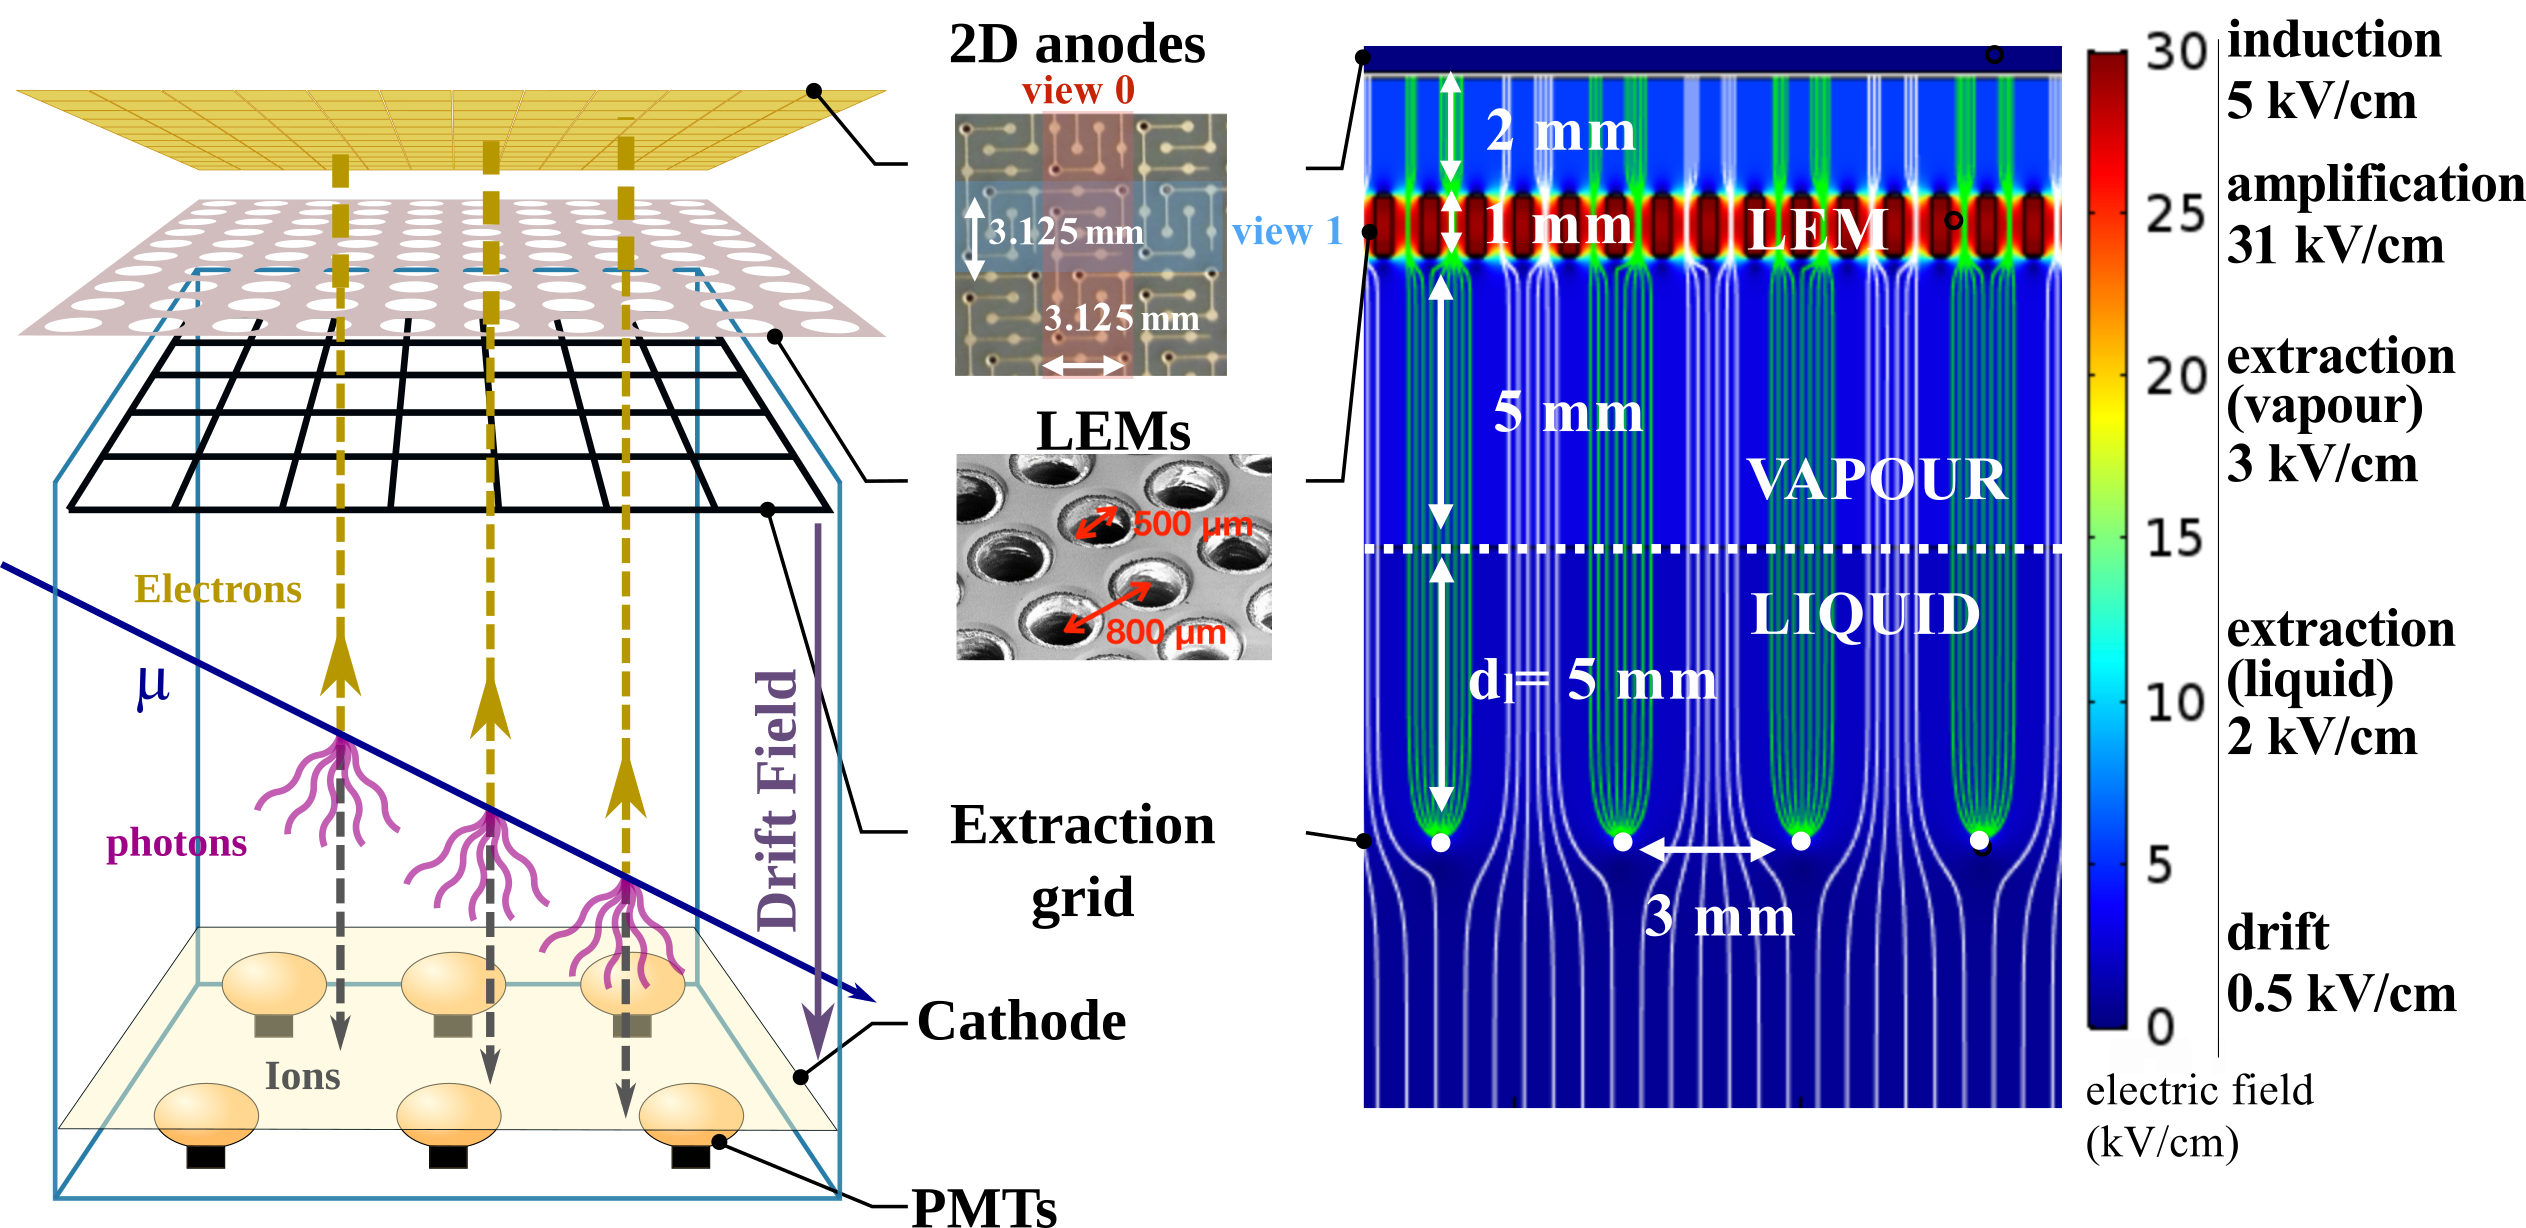
\includegraphics[width=\textwidth,keepaspectratio]{dlartpc_full.png}
      \caption[Schéma d'une chambre à projection temporelle à double phase d'argon liquide]{\label{fig::dlartpc}Schéma d'une chambre à projection temporelle à double phase d'argon liquide. La dérive des électrons se fait verticalement afin de pouvoir amplifier ces derniers à travers un ou plusieurs \acrfull{lem} situé dans une fine couche d'argon gazeux en haut du volume d'argon liquide.}
    \end{figure}
    
    Le projet \gls{wa105}, au \gls{cern}, prototype la technologie \gls{dlartpc} en vue de l'utiliser pour réaliser un modules de \SI{12}{\kilo\tonne} du détecteur lointain de \gls{dune} (\autoref{fig::wa105}). Un premier prototype de \TOO{} (\SI{4.2}{tonne}), construit et opéré au \gls{cern} entre 2016 et 2017, a prouvé que la technologie fonctionne avec une distance de dérive de \SI{1}{\meter} et une surface de lecture de charge de \SI{3}{\meter\squared}. Il a également testé et validé les choix technologiques utilisés pour la réalisation démonstrateur de \protodp{}; il a permis de souligner quelques difficultés techniques, notamment sur la tenue en tension des \glspl{lem}, qui ont pu être prises en compte pour la réalisation de ce démonstrateur de \SSS{} (\SI{300}{\tonne} d'argon liquide). Ce dernier, construit au \gls{cern} et qui prendra des données cosmiques à partir du mois d'août 2019, a pour but d'évaluer la capacité d'une \gls{dlartpc} de plusieurs centaines de tonnes à répondre aux besoins de \gls{dune} en terme de ratio signal/bruit, de résolution spatiale, de résolution en énergie, ainsi que développer les techniques de construction et d'exploitation d'une \gls{dlartpc} de plusieurs kilo tonnes.

    \begin{figure}[htbp]
      \centering
      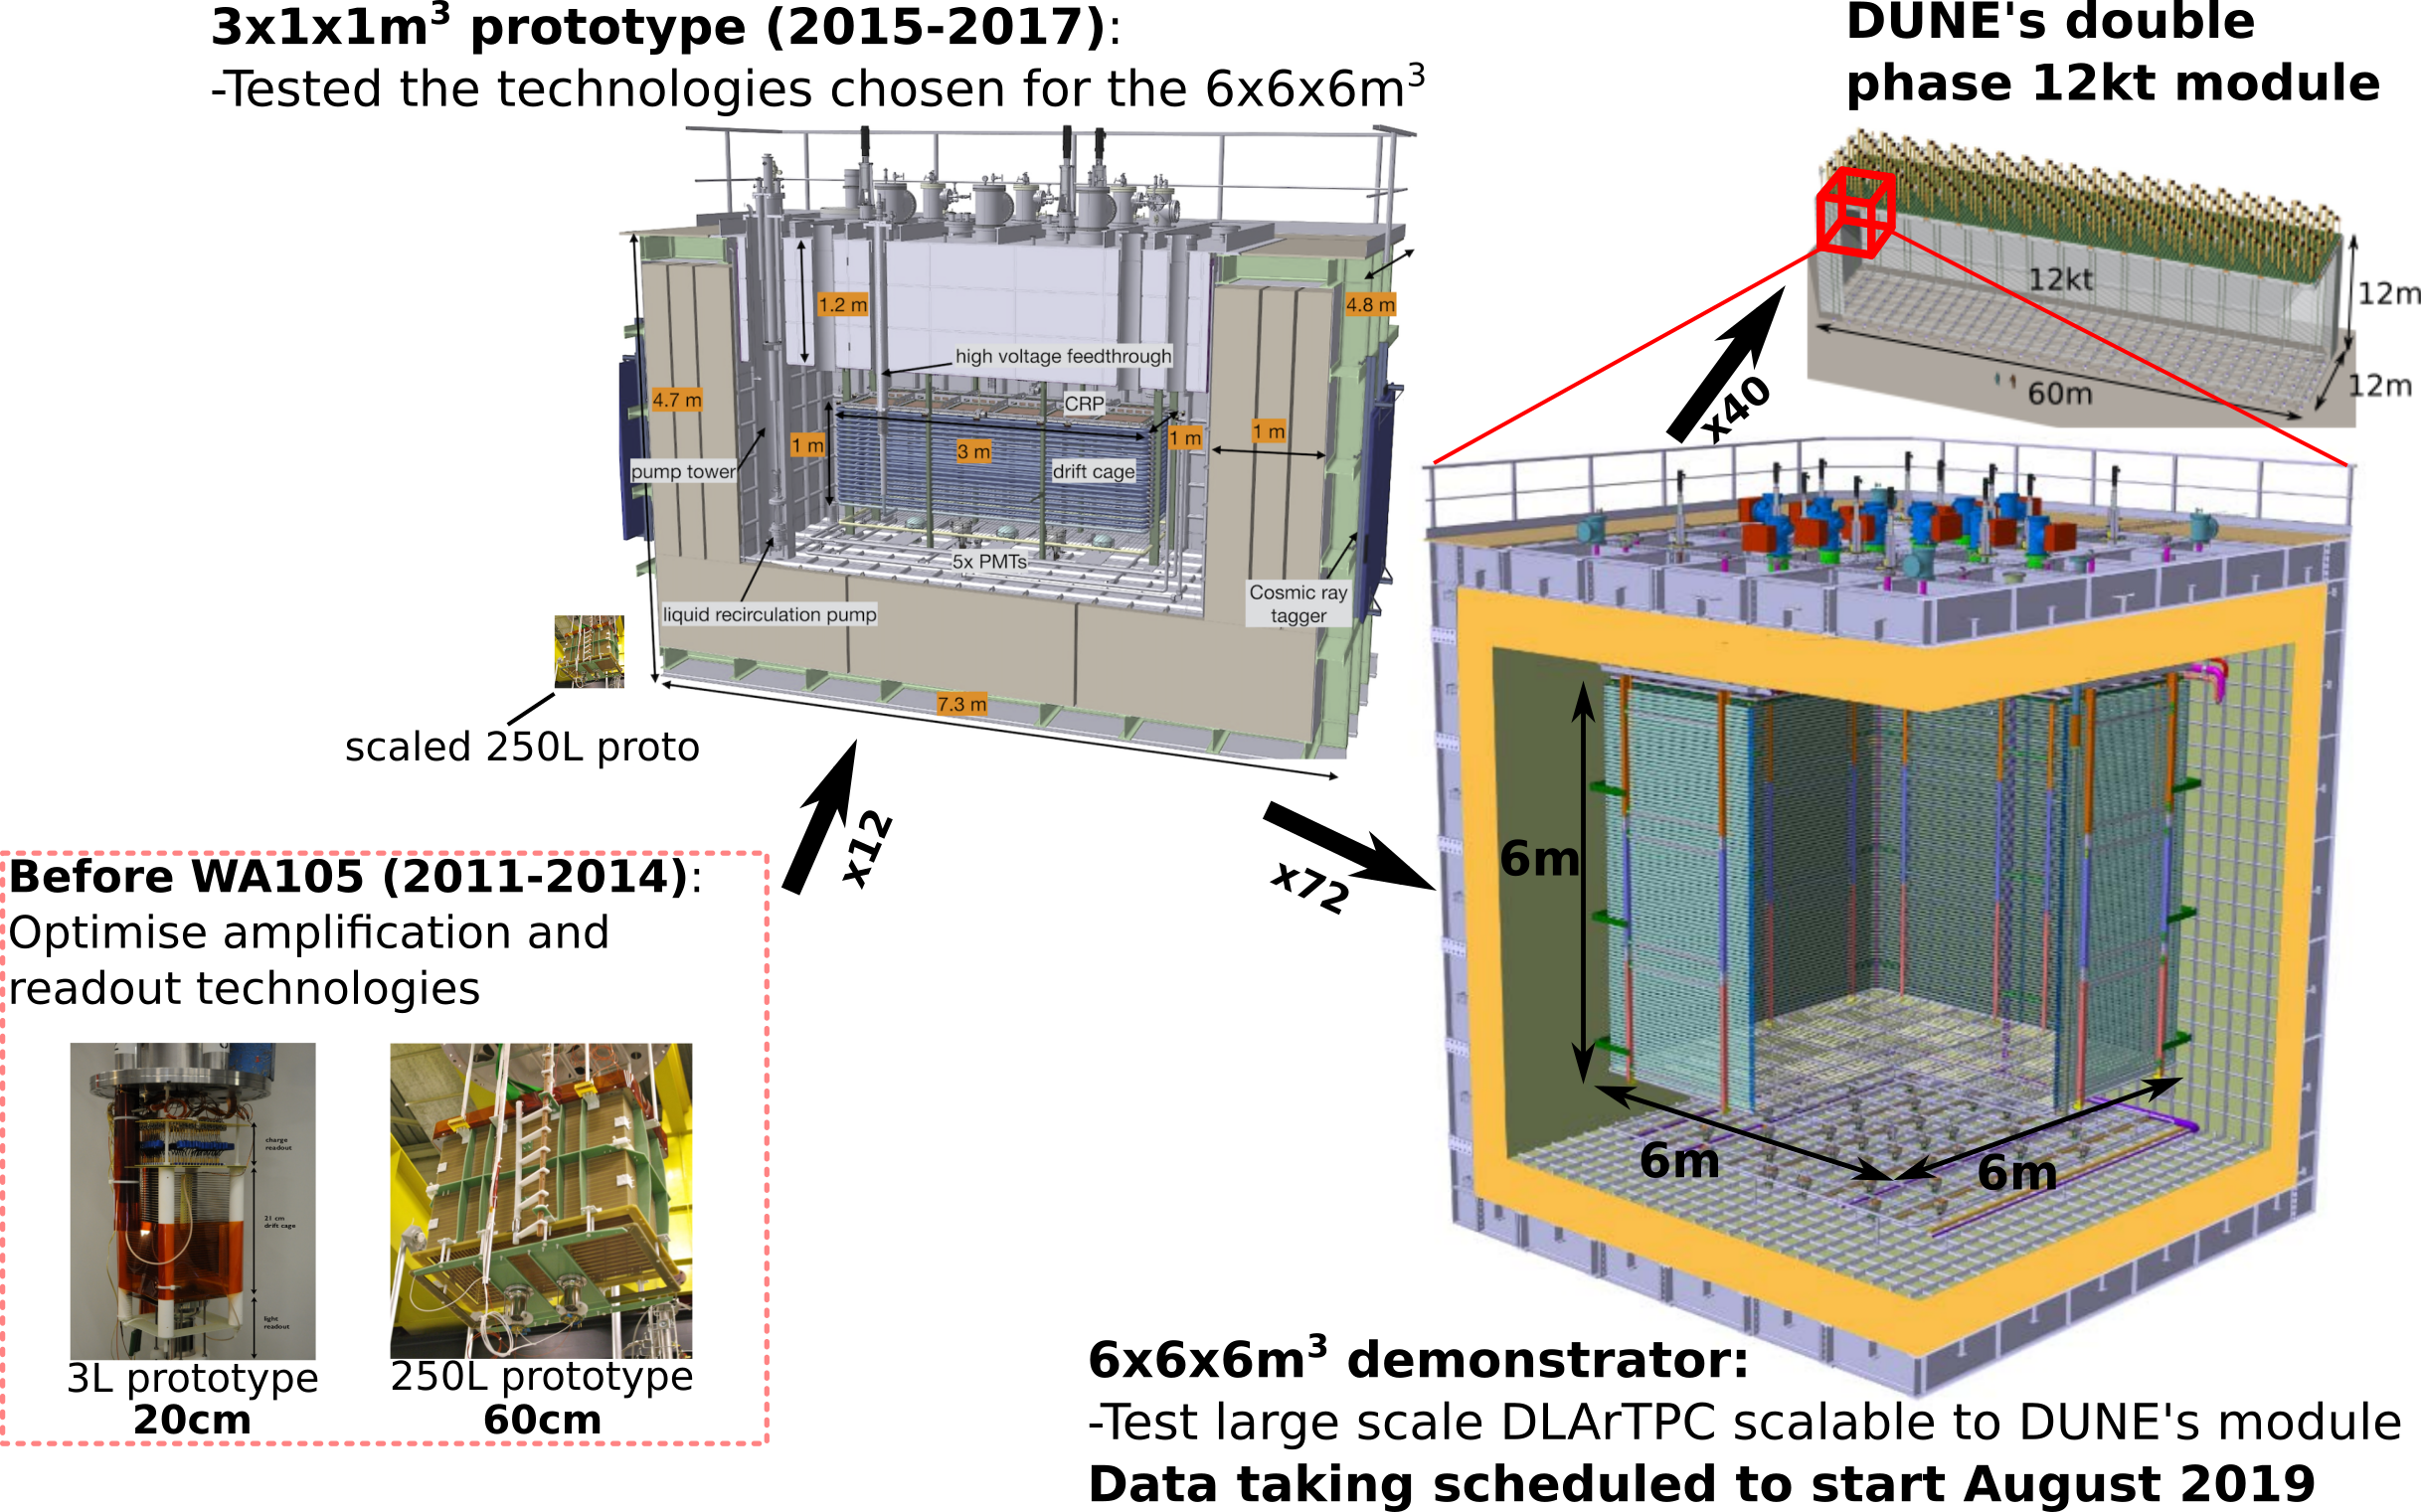
\includegraphics[width=\textwidth,keepaspectratio]{wa105_scale.png}        
      \caption[Le projet WA105]{\label{fig::wa105}\gls{wa105} et de sa place dans le développement de la technologie \gls{dlartpc}.}
    \end{figure}

    Nous commencerons ce chapitre en détaillant le design et les objectifs du prototype \TOO{}, dont les résultats sont analysés au \autoref{chap::5}. Nous détaillerons ensuite le démonstrateur \SSS{}. Nous continuerons avec une description détaillé des processus propres aux \gls{dlartpc} de \gls{wa105} puis avec l'état de l'art de cette technologie, et nous finirons par décrire les différents processus physiques impliqués dans l'ionisation, la dérive, l'extraction, l'amplification et la collection des électrons dans l'argon liquide.

  \section{Les DLArTPC de WA105}

    \subsection{Avantages et inconvénients de la technologie DLArTPC}

%      Le principe de base d'une \gls{tpc} est l'ionisation d'un milieu homogène par le passage de particules chargées et la collection des électrons ainsi créés sur une surface capable de reconstruire une information en deux dimensions., en générale, a plusieurs avantages:
%      \begin{itemize}
%        \item[$\bullet$] Toutes les interactions ont lieu dans un volume homogène et continue, sans zones mortes.
%        \item[$\bullet$] Le gaz ou le liquide remplissant ce volume est à la fois la cible et le milieu de détection.
%        \item[$\bullet$] L'information 3D des traces est reconstruite sans ambiguïté.
%        \item[$\bullet$] Il est possible de séparer plusieurs traces même quand la densité de trace est importante, permettant l'étude d'interactions complexes.
%        \item[$\bullet$] Il est possible de reconstruire la charge déposée dans le milieu et d'utiliser le dépôt d'énergie par unité de longueur pour identifier les particules.
%      \end{itemize}

      L'amplification du signal permet la détection d'événements plus bas en énergie. Avec un bruit électronique de moins de \numprint{2000} électrons (correspondant au bruit électronique des anodes du prototype de \TOO{}) et un gain de 20, un rapport signal sur bruit de \numprint{240} peut être atteint pour un muon au minimum d'ionisation et une dérive de \SI{1}{\meter}.

      Cette distance de dérive correspondant à la distance entre la trace de la particule traversant le détecteur et le dispositif de lecture des électrons. Dans une \gls{lartpc}, la présence d'impuretés dans l'argon liquide va influencer la valeur maximale de cette distance au dessus de laquelle une trace est détectable. Ces impuretés vont absorber une partie des électrons de dérive (plus de détails en \autoref{sec::purity}), et plus la distance de dérive est grande plus le nombre d'électrons lus est faible. Le gain d'une \gls{dlartpc} permet de diminuer le seuil de détection et donc d'augmenter la distance de dérive maximum. Ceci permet d'avoir un volume utile plus grand et ininterrompu.

      Une amplification permet également de travailler avec des canaux de lecture plus fins, étant donné que le seuil en énergie peut être plus bas. Ceci peut alors améliorer la résolution spatiale sur deux dimensions.

      Concernant les inconvénients, il y en a deux principaux. Le premier concerne la précision sur la mesure de l'énergie. En effet, le processus d'avalanche de Townsend dépend exponentiellement de la densité du gaz et de l'épaisseur des \glspl{lem} servant à l'amplification (voir équation \autoref{eq::townsend}). Des variations de l'ordre du pourcent de l'un de ces paramètres peut entraîner une variation de l'ordre de la dizaine de pourcent sur le gain. L'effet de l'épaisseur des \glspl{lem} est discutés en détail en \autoref{sec::epaisseur}. Concernant la densité, le \TOO{} a montré qu'il est possible de travailler à des conditions thermodynamiques très stables (variations de l'ordre du pour mille, voir \autoref{sec::slow_control}). Le second inconvénient est l'effet de charge d'espace, et concerne essentiellement les grands prototypes en surface. La vitesse de dérive des ions dans l'argon liquide est bien plus faible que celle des électrons. Une accumulation d'ions dans le volume liquide peut donc entraîner une modification du champ électrique et ainsi déformer les traces. Ce processus est vrai pour les \glspl{lartpc} simple phase également, mais il peut être accru dans les \glspl{dlartpc} à cause du retour dans le liquide des ions produits lors de l'amplification\cite{Romero2016}. Toutefois, si le taux d'événements est faible, la plupart de ces ions seront évacués entre deux événements. Ce sera la cas dans \gls{dune}, qui sera protégé des rayons cosmiques et qui détectera des événements rares, c'était le cas dans le \TOO{}, qui a une volume suffisamment petit, mais ce n'est pas le cas des prototypes de \protodp{}.

    \subsection{Le prototype de \TOO{}}\label{sec::TOO-intro}

      \begin{figure}[htbp]
        \centering
        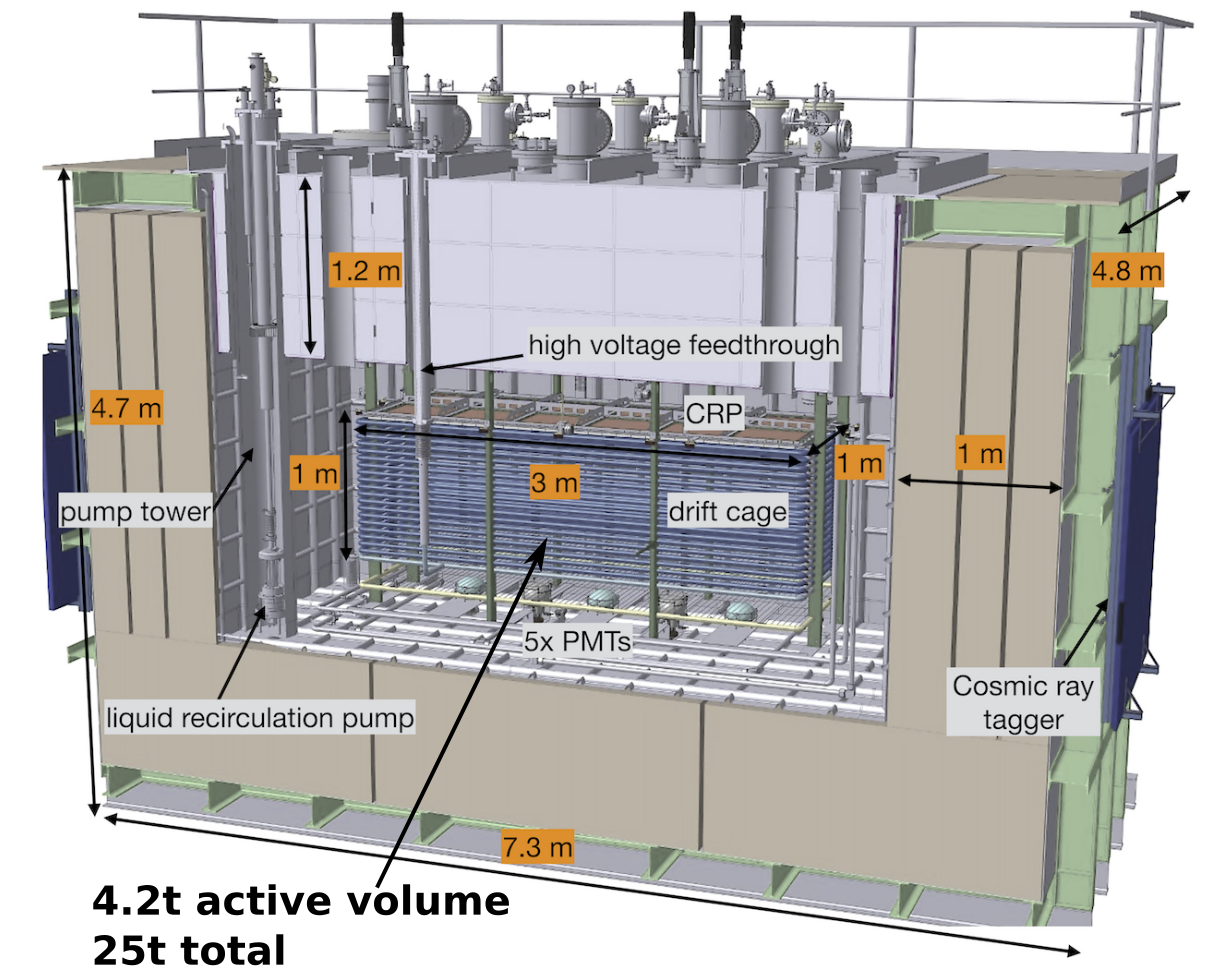
\includegraphics[width=0.8\textwidth,keepaspectratio]{311_2.png}        
        \caption[Schéma du prototype de \TOO{}]{\label{fig::311}Schéma du prototype de \TOO{}.}
      \end{figure}

      Le \TOO{}, construit et exploité entre 2016 et 2017, avait deux objectifs principaux :
      \begin{itemize}
        \item[$\bullet$] Prouver que la technologie \gls{dlartpc} fonctionne à l'échelle de plusieurs tonnes avec une dérive de \SI{1}{\meter} et une surface de lecture de plusieurs \si{\meter\squared}. Il devait donc réussir à voir des traces traversant l'ensemble de la hauteur du détecteur, et reconstruire leurs différentes caractéristiques (énergie, angles, positions...). Il devait aussi étudier la stabilité du gain sur la surface de lecture ainsi que son comportement en fonction du temps et en fonction des différents champs électriques appliqués.
        \item[$\bullet$] La plupart des choix techniques faits pour la construction du \TOO{} sont identiques à ceux fait pour le \SSS{}, notamment le cryostat, l'approvisionnement en argon, les \glspl{pmt}, le \gls{crp}), et l'électronique de lecture. Le \TOO{} a donc servi à tester ces choix afin d'anticiper d'éventuels problèmes.
      \end{itemize}
      
      La \autoref{fig::trace_311} montre deux traces traversant toute la hauteur du \TOO{}, une gerbe électromagnétique et un muon. Le champ d'amplification était alors de \SI{29}{\kilo\volt\per\centi\meter}, correspondant à un gain attendu de 9. Le comportement du gain est étudié en détail dans le \autoref{chap::5} en utilisant des muons cosmiques, dont le dépôt de charge attendu sert de référence (voir \autoref{sec::ionisation}).

      \begin{figure}[htbp]
        \centering
        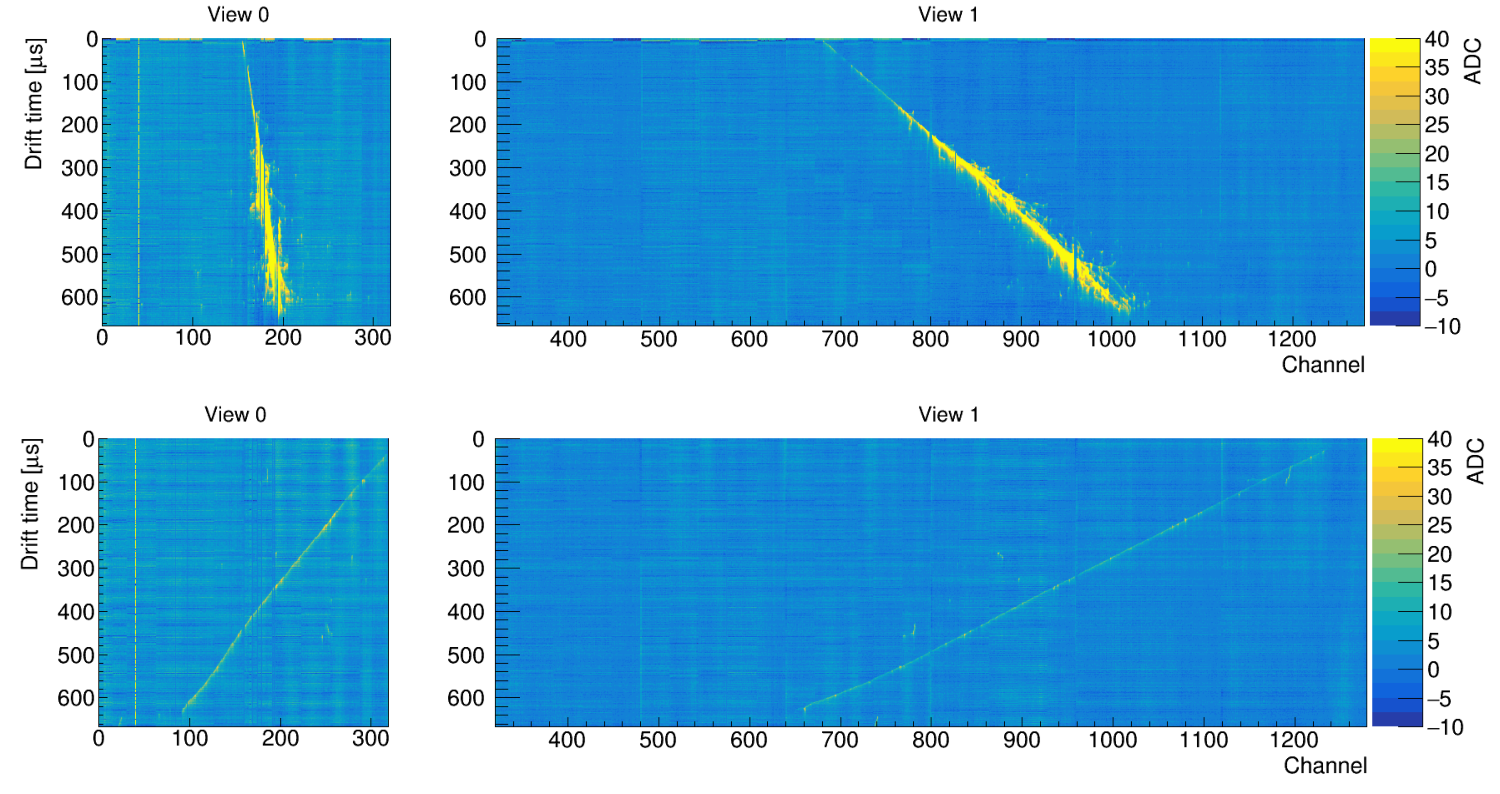
\includegraphics[width=\textwidth,keepaspectratio]{311_event}        
        \caption[Quelques événements vus dans le  \TOO{}]{\label{fig::trace_311}Une gerbe électromagnétique et un muon cosmique vus dans le \TOO{}. L'amplification était alors de \SI{29}{\kilo\volt\per\centi\meter}.}
      \end{figure}

      Comme il est expliqué au \autoref{chap::5}, des problèmes de tenue en tension durant les opérations ont grandement limité la quantité et la qualité de données. Ces problèmes, surtout dus au design des \glspl{lem} et à la tension mécanique des fils de la grille d'extraction, ont été pris en compte dans la conception des \glspl{crp} du \SSS{}.

      Tous les détails techniques présentés ici sont tirés de \cite{Aimard2018}. Le prototype de \TOO{} est présenté en \autoref{fig::311}. Ses dimensions extérieures sont de $\numprint{7.3}\times\numprint{4.7}\times\SI{4.8}{\meter\cubed}$. Le volume interne du cryostat
      est d'environ \SI{23}{\meter\cubed}. Ce dernier est constitué d'une couche d'acier inoxydable ondulé, capable d'absorber les déformations dues aux contractions thermiques, et d'un isolant d'un mètre d'épaisseur. Le volume actif de \TOO{} est délimité par la cage de dérive , fournissant le champ de dérive homogène de \driftfield{}, la cathode en bas de la cage de dérive et le \gls{crp}, en haut de la cage de dérive. La cage de dérive est un assemblage vertical de vingt anneaux creux de section de \SI{34}{\milli\meter} d'acier inoxydable espacés de \SI{5}{\centi\meter}. Ces anneaux sont reliés entre eux par des résistances de \SI{100}{\ohm} (à température ambiante), le tout assurant un champ de dérive uniforme dans les \SI{3}{\meter\cubed} du volume actif. La cathode est une grille faite de tubes d'acier inoxydables de \SI{4}{\milli\meter} de diamètre répartis espacés de \SI{2}{\centi\meter}, fixée à l'anneau du bas de la cage de dérive. Sous la cathode sont situés cinq \glspl{pmt} servant à la détection de la lumière de scintillation émise lors de l'ionisation de l'argon, utilisée pour déterminer le temps initial des événements. Ces \glspl{pmt} ont également servi de déclencheur. 

      L'ensemble est suspendu au top-cap, couvercle isolant de \SI{1.2}{\meter} d'épaisseur fermant le cryostat. Le \gls{crp} n'est pas solidaire de la cage de dérive et, grâce à trois câbles traversant le top-cap, peut être positionné précisément en fonction du niveau d'argon liquide. Le top-cap est traversé par les cheminées permettant d'amener la haute tension aux différents éléments et de récupérer les données des différents capteurs, que ce soit les anodes de lectures, les \glspl{pmt}, ou les capteurs de température, de pression et de niveau d'argon permettant la surveillance en temps réel des conditions à l'intérieur du cryostat. A l'extérieur du cryostat, aux deux extrémités du volume total, se trouvent des plans \gls{crt} pouvant servir de déclencheur externe capable de sélectionner des événement quasi-horizontaux.

      Le remplissage d'argon liquide du cryostat se fait en quatre étapes. La première étape, appelée "boucle ouverte", consiste à injecter de l'argon gazeux à température ambiante à un débit de \SI{2}{\liter\per\second} en bas du cryostat par quatre tuyaux, chacun percés de trois ouvertures. Ceci permet de pousser l'air présent uniformément vers le haut du volume où il est évacué. Le processus continue après que tout l'air ait été évacué jusqu'à ce que les concentrations d'impuretés se stabilisent, ce qui correspond environ à 80 fois le volume du cryostat. Commence alors la seconde étape : la circulation d'argon continue mais ce dernier n'est pas évacué. Il passe à travers un purificateur et est réinjecté dans le cryostat afin de continuer à diminuer les impuretés. Ceci prend une centaine de volumes de cryostat avec un débit de \SI{4}{\liter\per\second}. La troisième étape est le refroidissement, fait en injectant aux quatre coins du bas du cryostat un mélange d'argon gazeux à température ambiante et d'argon liquide à \SI{87}{\kelvin}, pour un débit de \SI{500}{\liter\per\minute} et \SI{1266}{\liter\per\minute} respectivement. Il faut environ cinq jours pour arriver à la température à \SI{170}{\kelvin}, après quoi la quatrième étape, le remplissage, peut commencer. Durant les opérations, l'argon liquide est continûment prélevé, purifié et réinjecté par une pompe située dans un coin en bas du cryostat. Deux volumes par jour circulent ainsi dans le cryostat. De plus, l'argon gazeux est également continûment récupéré, liquéfié et réinjecté dans le cryostat. 

      \begin{figure}[htbp]
        \centering
        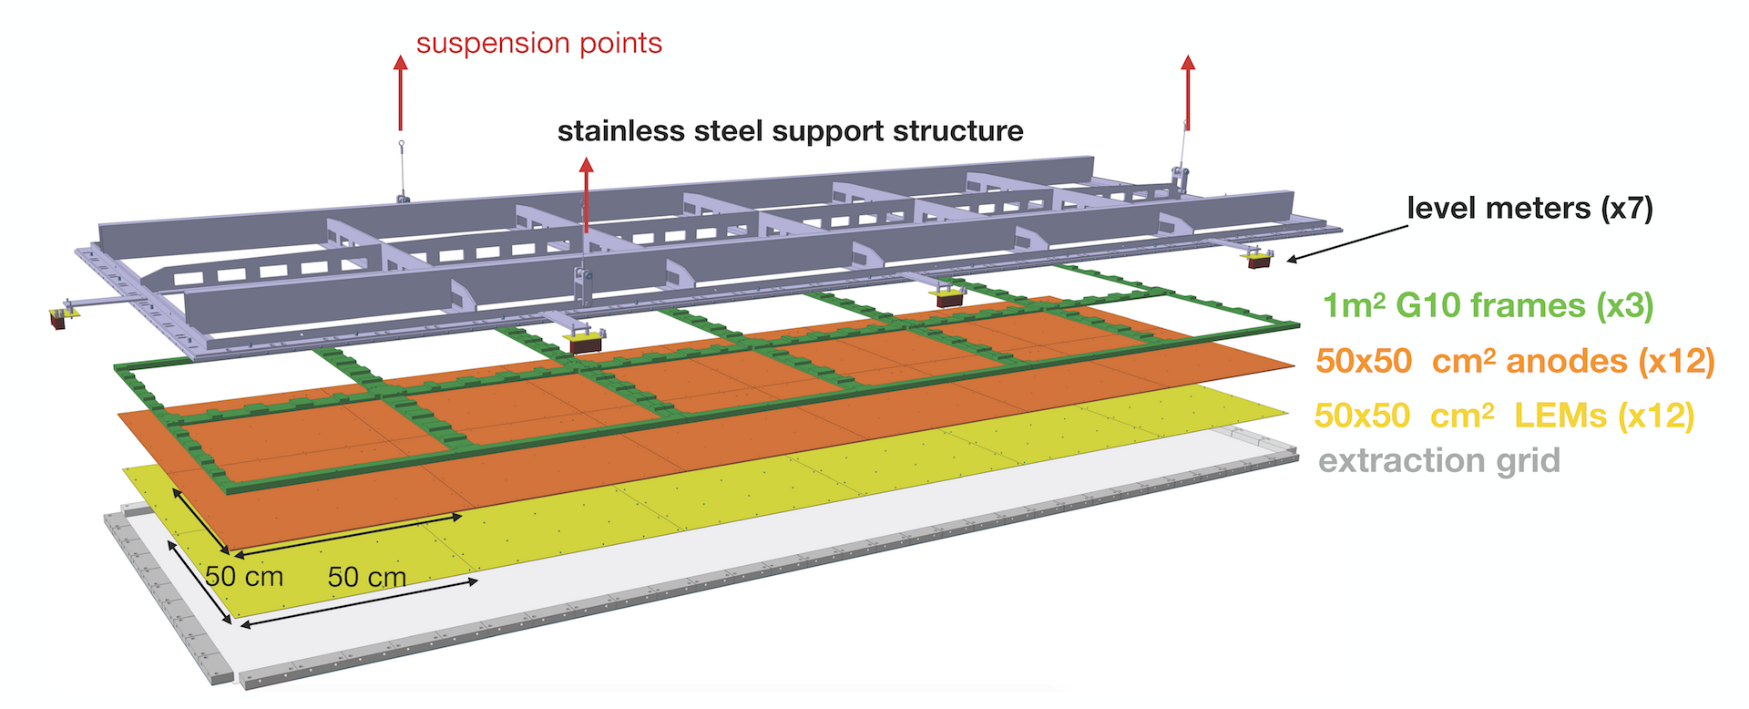
\includegraphics[width=\textwidth,keepaspectratio]{crp_exp.png}        
        \caption[Schéma explosé du CRP du \TOO{}]{\label{fig::crp_exp}Schéma explosé du \gls{crp} du \TOO{}.}
      \end{figure}

      Une vue explosée du \gls{crp} du \TOO{} est présentée en \autoref{fig::crp_exp}. Ce dernier est composé de 12 \gls{las} de $50\times\SI{50}{\centi\meter\squared}$,  espacés de \SI{0.5}{\milli\meter}, et d'une grille d'extraction constituée d'un maillage carré de fils d'inox tendus à \SI{3}{\newton\per\meter}. Ces fils sont espacés de \SI{3.125}{\milli\meter} ce qui est égal à la taille des canaux de lecture des anodes. Chaque anode est munie de $160\times160$ canaux de lecture horizontaux, avec une impédance de \SI{160}{\pico\farad\per\meter}. Les anodes sont reliées entre elles par des nappes et des connecteurs KEL permettant de former des canaux de lecture continus de \SI{1}{\meter} et \SI{3}{\meter}. Le bruit de fond correspondant aux \SI{160}{\pico\farad\per\meter} est inférieur à \numprint{2000} électrons dans les canaux de \SI{3}{\meter}\cite{Aimard2018}. Chaque \gls{lem} est fixé à \SI{2}{\milli\meter} sous son anode par 29 vis en \gls{peek} munies d'entretoises en MACOR. Les zones des \glspl{lem} autour de ces vis et des connecteurs haute tension sont dépourvues de cuivre et de trous d'amplification, de même que le bord du \gls{lem}. Ceci réduit la surface active du \gls{lem} à 96\,\%. L'impact de ces zones mortes sur la collection de charge est étudiée en \autoref{sec::dead_zones}. Les différents éléments du \gls{crp} sont fixés sur un cadre en G10, dont le coefficient de dilatation thermique est proche de celui des \glspl{las} le tout monté sur un cadre en inox muni de détecteurs de niveau d'argon, permettant de mesurer en direct la position du \gls{crp} par rapport à l'interface liquide-gaz. Le cadre en inox est suspendu au top-cap par trois câbles permettant d'ajuster la position verticale du \gls{crp}. La \autoref{fig::dlartpc} présente une vue en coupe du champ électrique à travers le \gls{crp} pour les tensions nominales d'opération.

      L'emplacement de l'électronique de lecture est un des avantages de la \gls{dlartpc} sur la \gls{lartpc} simple phase : les cartes front-end sont situées en bas des cheminées, et profitent ainsi de la basse température du cryostats qui réduit le bruit électronique tout en pouvant être retirées pour maintenance durant les opérations sans avoir à ouvrir le top-cap. La numérisation des signaux quant à elle est faite à l'extérieur du cryostat. Les 320 canaux longs de \SI{3}{\meter} constituent la \textit{vue 0} du détecteur, tandis que les 960 canaux de \SI{1}{\meter} constituent la \textit{vue 1}. Chaque canal est découpé en \numprint{1667} bins de temps de \SI{0.4}{\micro\second} chacun, couvrant ainsi une fenêtre de \SI{667}{\micro\second}. La vitesse de dérive d'un électron dans l'argon liquide et un champ de \driftfield{} étant de \SI{1.63}{\milli\meter\per\micro\second} (vir \autoref{sec::vitesse_derive}) ce temps correspond à une distance de \SI{1.09}{\meter}. Chaque canal est numérisé avec une résolution de 12 bits, couvrant \SI{1200}{\femto\coulomb}.

    \subsection{Le démonstrateur de \SSS{} de proto\texorpdfstring{DU$\nu$E}{DUNE}-DP}

      \begin{figure}[htbp]
        \centering
        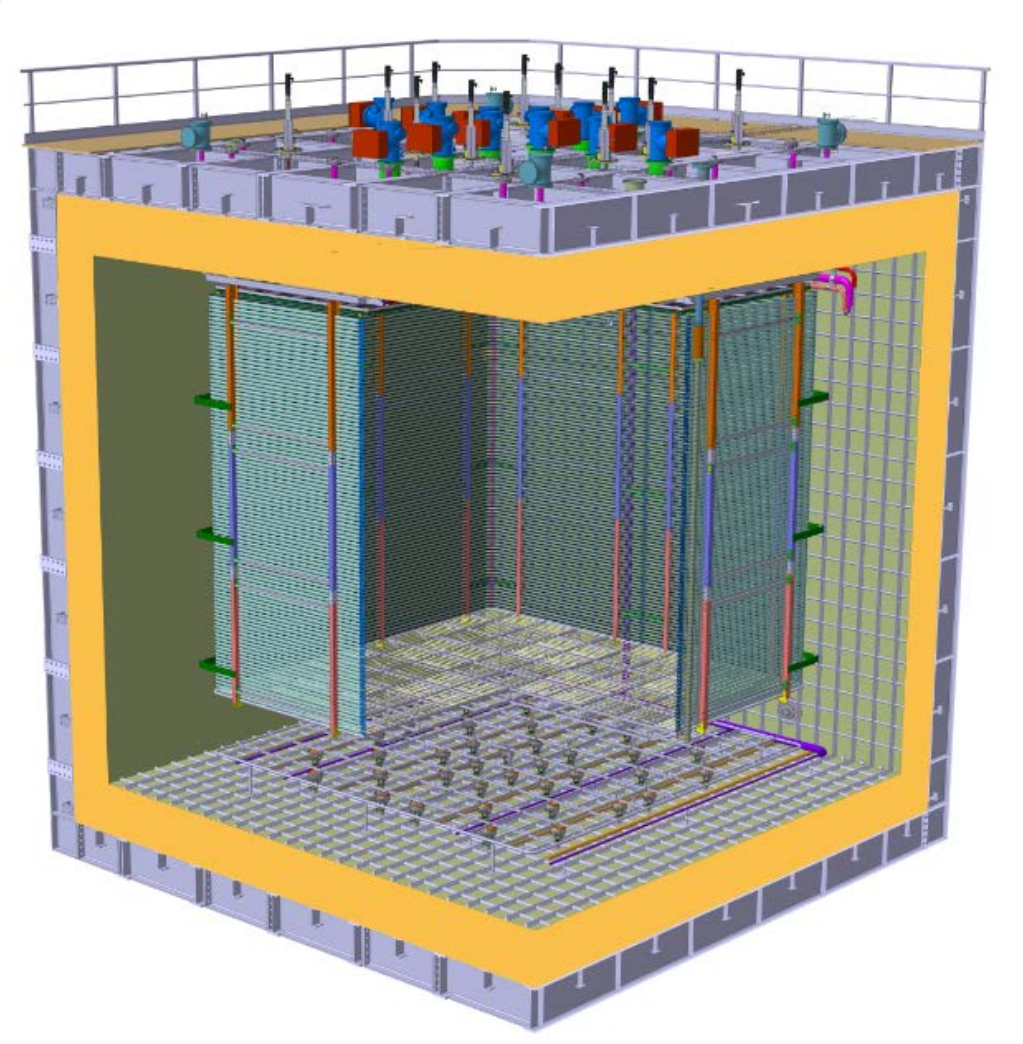
\includegraphics[width=0.8\textwidth,keepaspectratio]{666.png}        
        \caption[Schéma du démonstrateur de \SSS{}]{\label{fig::666}Schéma du démonstrateur de \SSS{}.}
      \end{figure}

      Le design actuel du futur module de \SI{12}{\kilo\tonne}\cite{Acciarri2016a} de \gls{dune} implique que le \gls{crp} sera constitué d'un assemblage de $4\times20$ "briques élémentaires" de $\SI{3}{\meter}\times\SI{3}{\meter}$. Ces \glspl{crp} élémentaires, schématisés en \autoref{fig::crp_666}, ont un design très similaire à celui du \TOO{}, la différence principale étant, en plus de la dimensions, que le cadre en inox est remplacé par un cadre en Invar, moins sensible aux contractions thermiques. Le démonstrateur de \SSS{} a été spécifiquement réalisé pour tester, à l'échelle, un ensemble de 4 de ces briques élémentaires avec une distance de dérive de \SI{6}{\meter}. Ces objectifs principaux sont :
      \begin{itemize}
        \item[$\bullet$] Évaluer la capacité de la technologie \gls{dlartpc} à répondre aux besoin de \gls{dune} (\autoref{tab::FD-perf}) en matière de ratio signal/bruit ainsi qu'en terme de résolution, aussi bien spatiale qu'en énergie. Ceci requiert de montrer qu'il est possible d'atteindre un gain effectif égal ou supérieur à 20, homogène sur la surface des \glspl{crp}, et de le maintenir sur de longues durées.
        \item[$\bullet$] Développer/améliorer l'ensemble des techniques liées à la construction et à l'exploitation d'une \gls{dlartpc} à l'échelle de \gls{dune}, de l'assemblage du cryostat jusqu'aux logiciels de reconstruction.
      \end{itemize}
      Les performances du \SSS{}, qui commencera à prendre des données en cosmiques en août 2019, seront directement extrapolables aux dimensions de \gls{dune}.

      \begin{figure}[htbp]
        \centering
        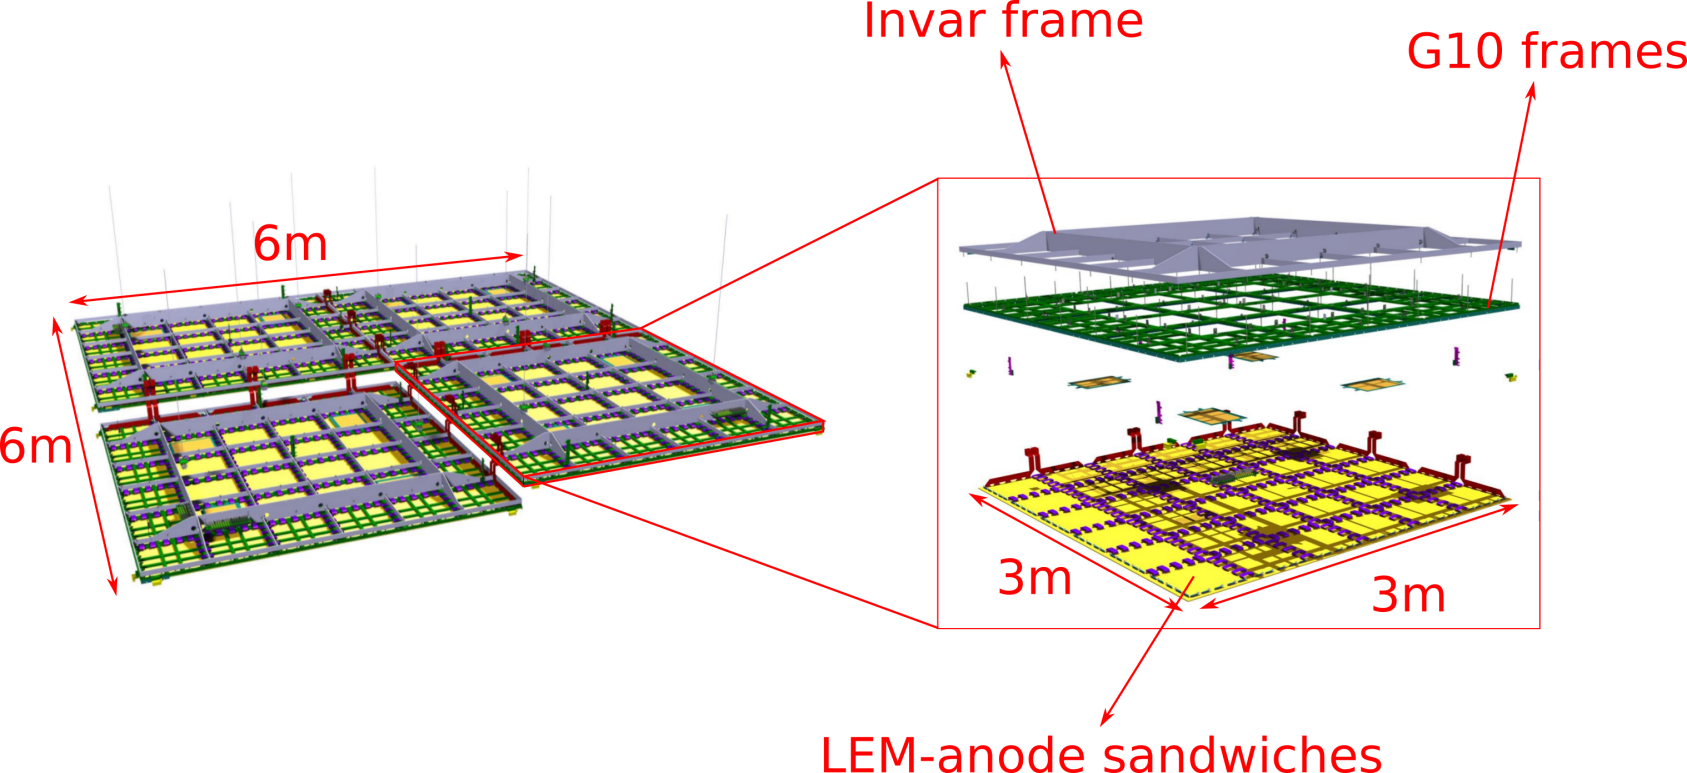
\includegraphics[width=\textwidth,keepaspectratio]{crp_666_complete.png}
        \caption[Schéma des CRPs du \SSS{}]{\label{fig::crp_666}Schéma des quatre \glspl{crp} du démonstrateur de \SSS{}.}
      \end{figure}

      \begin{figure}[htbp]
        \begin{subfigure}{0.48\textwidth}
          \centering
          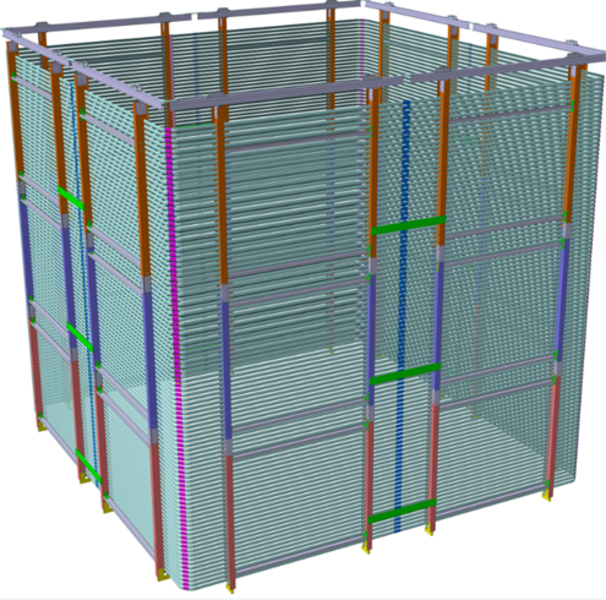
\includegraphics[width=\textwidth,keepaspectratio]{drift_cage_666.pdf}
        \end{subfigure}\hfill
        \begin{subfigure}{0.48\textwidth}
          \centering
          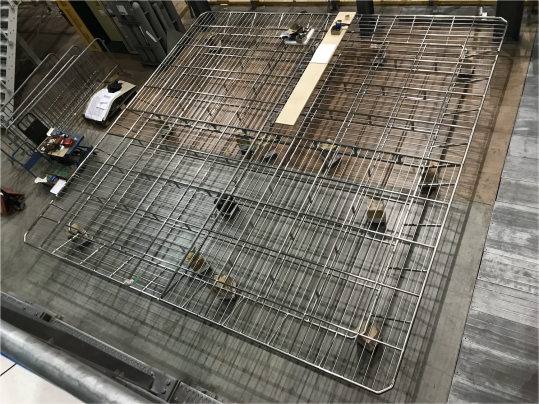
\includegraphics[width=\textwidth,keepaspectratio]{cathode_666.png}
        \end{subfigure}
        \caption[Cathode et cage de dérive du \SSS{}]{\label{fig::drift_cage_cathode_666}Schéma de la cage de dérive (droite) et test d'assemblage de la cathode (gauche) du \SSS{}.}
      \end{figure}

      La \autoref{fig::666} est une modélisation 3D du \SSS{}. Le cryostat et la cage de dérive ont été installés à la plateforme neutrino du \gls{cern} entre 2017 et 2018. Le design du cryostat est similaire à celui du \TOO{}. La cage de dérive (\autoref{fig::drift_cage_cathode_666}) est constituée de 8 modules verticaux de $\numprint{6.3}\times\SI{3}{\meter\squared}$, chacun constitué de trois sous-modules. Chaque module est formé d'un empilement de 98 profilés extrudés en aluminium séparés de \SI{6}{\centi\meter}, maintenus par des poutre en diélectrique. Les profiles d'un module est électriquement connecté aux profiles correspondant des deux modules adjacent, formant des anneaux entourant le volume actif. Chaque anneau est relié au suivant par deux diviseur de tension. La cathode (\autoref{fig::drift_cage_cathode_666}) est, comme le \gls{crp}, un assemblage de quatre modules de $3\times\SI{3}{\meter\squared}$. Les 36 \glspl{pmt} servant à la détection des photons de scintillations ont été installé sous le volume actif en février 2019. Afin de les protéger de la tension dans la cathode, une grille supplémentaire, à la masse a été installée entre les \glspl{pmt} et la cathode. Cette grille protégera également la membrane ondulée du cryostat en cas de décharge. 

      Le \SSS{} sera muni, comme le \TOO{}, de différents capteurs de pression, température et de niveau d'argon afin de surveiller les conditions dans le cryostat durant les opérations. Il sera également muni de deux capteur d'impuretés, un en bas du cryostat et un à une hauteur de \SI{2.5}{\meter}. La présence d'impureté peut dégrader le signal en absorbant une partie des électrons de dérive (voir \autoref{sec::purity}).

      Des tests de tenu en tension, avec les résultats du \TOO{}, ont permit de mettre en évidence et de résoudre un problème des \glspl{lem} (plus de détail en \autoref{sec::test_HT}) et de modifier le design initial de ces derniers afin d'atteindre des tensions stables à \SI{3.1}{\kilo\volt}, correspondant à un gain attendu de 20 (\autoref{fig::3L_gain}). Deux \glspl{crp} instrumentés avec 36 \gls{las} chacun ont été installés dans le cryostat entre fin 2018 et début 2019, après avoir subi des tests de tenue en tension et de stabilité dans une boite cryogénique dédiée (voir \autoref{sec::cold_box}). Par manque de temps, les deux autres \glspl{crp} n'ont pas été instrumentés, et sont munis de simples \glspl{pcb} et d'une grille d'extraction afin de fermer le champ électrique. Un de ces \glspl{crp} est néanmoins muni de quatre anodes et pourra ainsi étudier la collection de charge sans amplification. Il pourra ainsi avoir une mesure directe de l'efficacité d'extraction sur la charge lue. En effet, comme nous le montrons en \autoref{sec::extraction}, une partie des électrons peut être perdue lors de l'extraction du liquide vers le gaz. La prise de données avec des rayons cosmiques devrait commencer durant l'été 2019. 

      La \autoref{fig::pic_crp} est une photographie de l'intérieur du cryostat montrant les quatre \glspl{crp} vus de dessous, et une photographie du bas du volume durant l'installation des \glspl{pmt}. La \autoref{fig::cryogenie_666} montre les câblages sur le toit du cryostat et les installations cryogéniques.

      \begin{figure}[htbp]
        \centering
        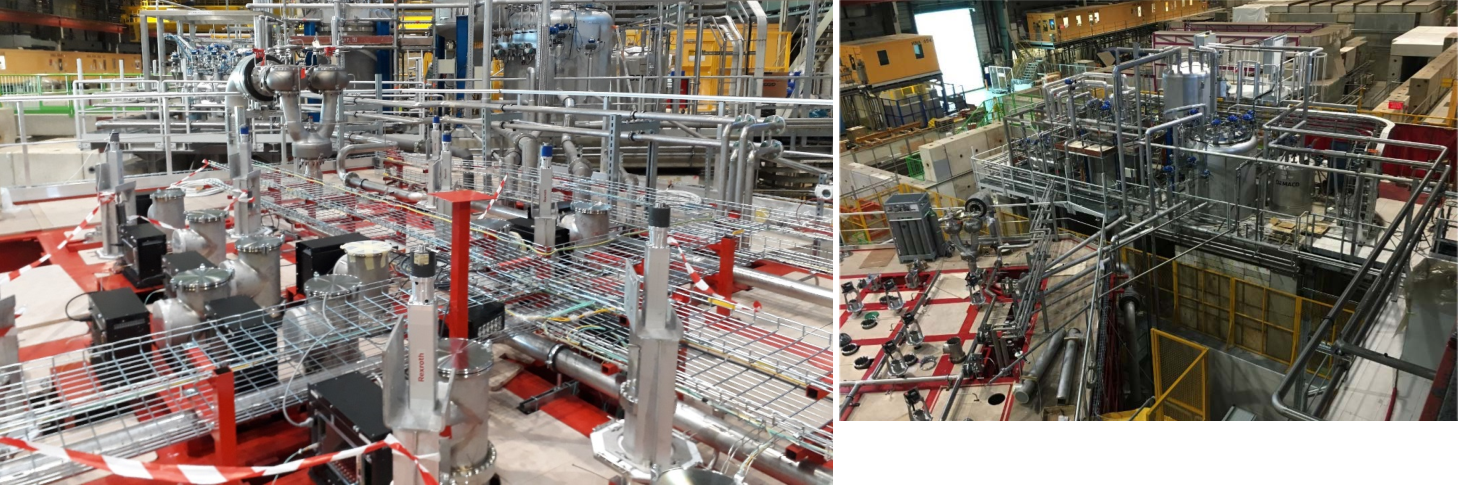
\includegraphics[width=\textwidth,keepaspectratio]{cryogenie_666.pdf}
        \caption[Câble et système cryogénique du \SSS{}]{\label{fig::cryogenie_666}Câble et système cryogénique du \SSS{}.}
      \end{figure}

      \begin{figure}[htbp]
        \centering
        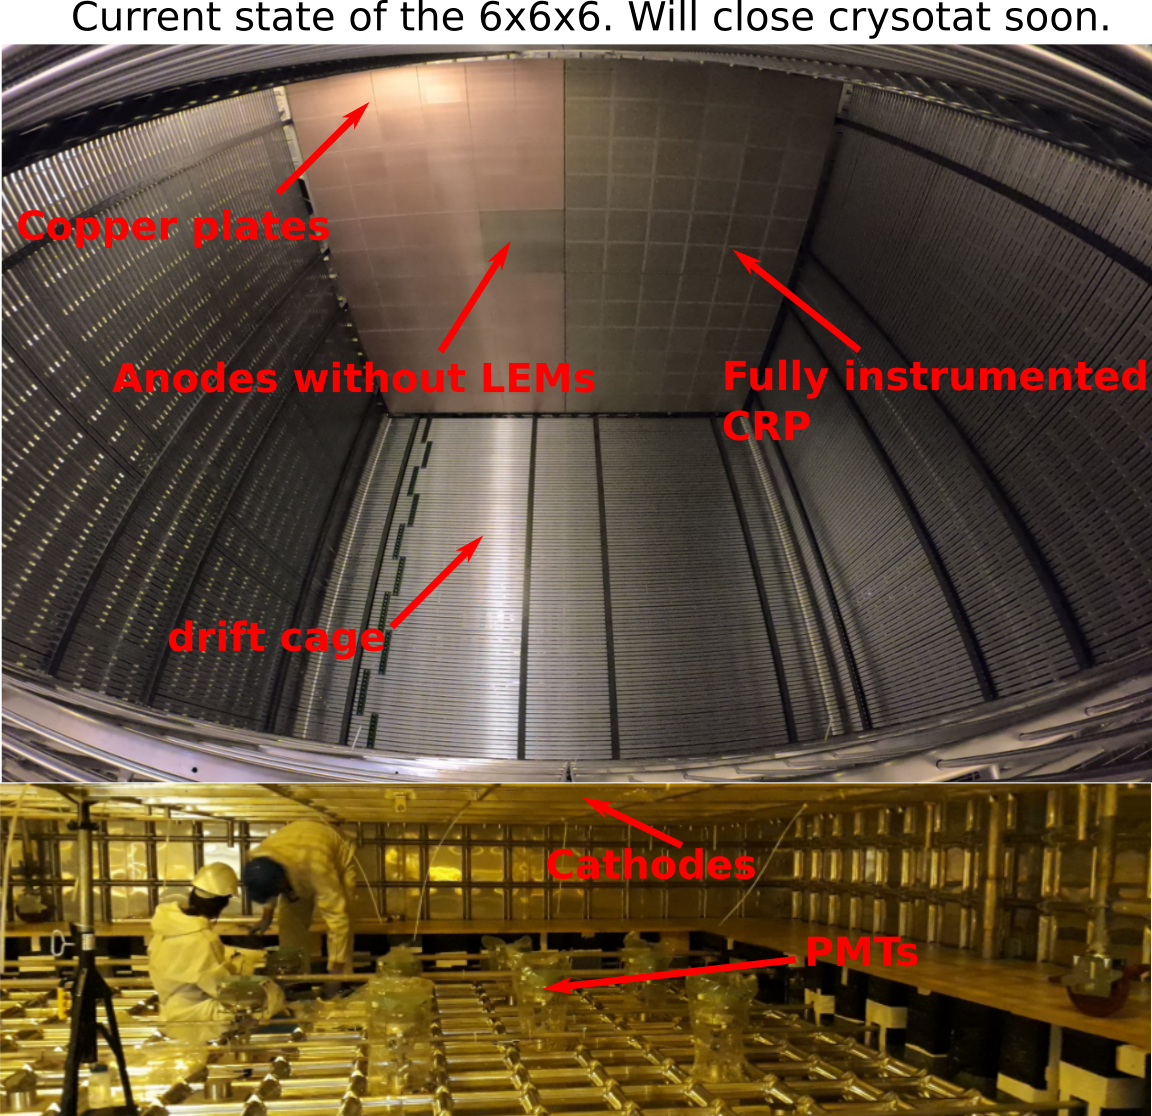
\includegraphics[width=\textwidth,keepaspectratio]{fisheye.png}        
        \caption[Photographie de l'intétrieur du démonstrateur de \SSS{}]{\label{fig::pic_crp}Photographies de l'intérieur du démonstrateur de \SSS{} (mars 2019). On y voit, en haut, les quatre \glspl{crp} dont deux sont instrumentés avec des \glspl{lem} et d'anodes, un non instrumenté et un muni de quatre anodes sans \glspl{lem}. Ce dernier pourra étudier la collection de charge sans amplification et ainsi avoir une mesure direct de l'efficacité d'extraction sur la charge lue. En bas sont visibles les cathodes et les \glspl{pmt}, alors en cours d'installation.}
      \end{figure}

  \section{Fonctionnement d'une DLArTPC utilisant des LEMs}\label{sec::dlartpc}
 
      La technologie à double phase a été proposée par A. Rubbia\cite{Rubbia2004} en 2004. Un premier prototype de \threeL{} avec une longueur de dérive de \SI{21}{\centi\meter} a été testé dans les années 2010, et a permis de définir les technologies d'amplification et de collection de charge\cite{Cantini2013} et d'évaluer les performances en terme de gain et de stabilité\cite{Cantini2014}.

    \subsection{Avalanche de Townsend}\label{sec::townsend}
      
      Le principe de l'amplification de charges dans un gaz est celui de l'avalanche de Townsend, nommé d'après John Sealy Townsend qui l'a étudié début 1900\cite{Townsend1910}. Il a été utilisé dans la détection de particules depuis sa découverte, notamment dans les compteurs Geiger et les \glspl{pmt}. Un électron présent dans un gaz va être accéléré par l'application d'un champ électrique. Si ce dernier est assez intense, l'électron acquière suffisamment d'énergie pour ioniser le gaz, créant plus d'électrons. Ces électrons sont accélérés à leur tour, ionisant le gaz et créant encore plus d'électrons. Ce processus est clairement exponentiel, et le gain $G$ résultant s'écrit, si l'on néglige les recombinaisons avec les ions :
      \begin{equation}\label{eq::townsend_compact}
        G = e^{\alpha\times d}
      \end{equation}
      où $d$ est la distance sur laquelle les électrons sont amplifiés et $\alpha$ est le premier coefficient de Townsend, indiquant le nombre d'ionisation par centimètre. Dans les \glspl{dlartpc} de \gls{wa105}, $d$ correspond à l'épaisseur des \glspl{lem}. Le coefficient de Townsend dépend de la nature du gaz ainsi que de sa densité, et du champ électrique appliqué. Une forme analytique a été proposée par T. Aoyama en 1985\cite{Aoyama1985}:
      \begin{equation}\label{eq::townsend_coef}
        \alpha = A\rho e^{-B\rho/E}
      \end{equation}
      où $\rho$ est la densité du gaz, $A$ et $B$ dépendent de la nature du gaz et $E$ est le champ électrique. L'équation \eqref{eq::townsend_compact} devient
      \begin{equation}\label{eq::townsend}
        G = e^{A\rho  de^{-B\rho /E}}.
      \end{equation}

      Dans les \glspl{dlartpc} de \gls{wa105}, il est impossible de mesurer directement $G$ à cause de la perte possible d'électrons avant et après l'amplificateur (plus de détails en \autoref{sec::efficacites}). On utilise plutôt le gain effectif $G_{eff}$ défini comme
      \begin{equation}\label{eq::gain_eff}
        G _{eff}= \mathcal{T}G
      \end{equation}
      où $\mathcal{T}$ est un facteur compris entre 0 et 1 et correspond à la "transparence" aux électrons du \gls{crp}. 

      Dans les \glspl{dlartpc} de \gls{wa105}, l'amplificateur est constitué d'un ou plusieurs \glspl{lem} placés à \SI{0.5}{\milli\meter} au dessus de l'interface liquide-gaz. Un \gls{lem}, montré en \autoref{fig::lem}, est une plaque d'epoxy \gls{fr4} de \SI{1}{\milli\meter} d'épaisseur, recouverte sur chaque face d'une mince couche de cuivre (quelques dizaines de \si{\micro\meter}), et percée de trous de \SI{0.5}{\milli\meter} de diamètre espacés de \SI{0.8}{\milli\meter}, entourés d'un anneau sans cuivre appelé RIM, de quelques dizaines de \si{\micro\meter}. Une différence de potentiel entre les deux faces du \gls{lem} permet de générer le champ d'amplification. La technologie du \gls{lem} présente plusieurs avantages comparée aux GEM et aux micro-mégas : un \gls{lem} de \SI{1}{\milli\meter} d'épaisseur peut être produit industriellement, est fait avec des matières premières standards et a un faible coup par unité de surface Enfin, il est peu sensible à la contraction thermique impliquée par la cryogénie de la technologie \gls{dlartpc}.

    \subsection{Extraction des électrons du liquide vers le gaz}\label{sec::extraction}

      \begin{figure}[htbp]
        \centering
        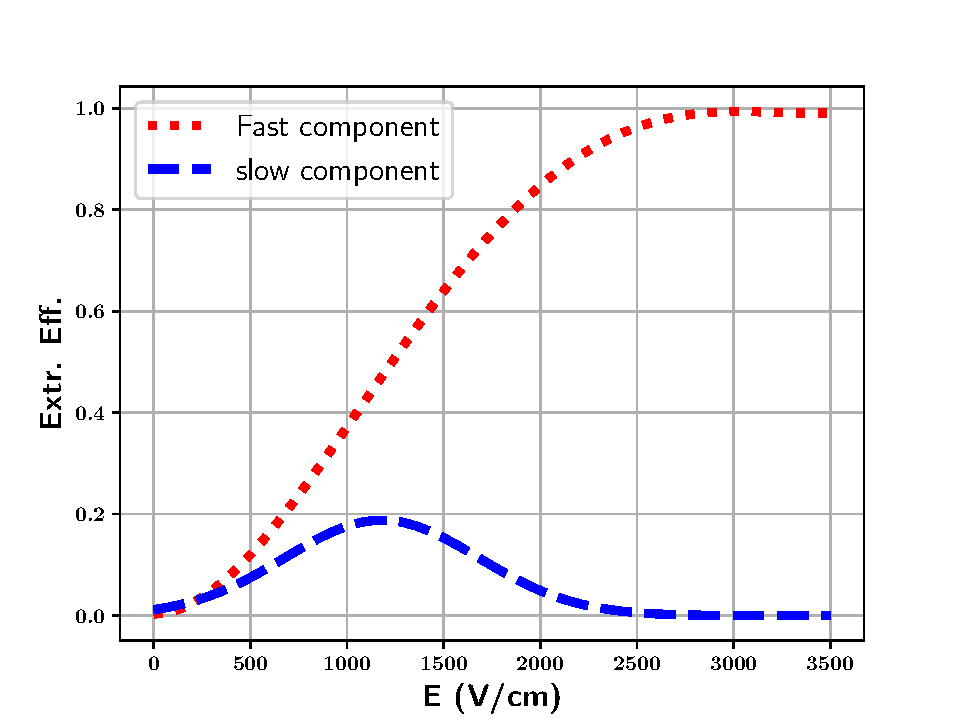
\includegraphics[width=0.8\textwidth,keepaspectratio]{eff_vs_E.pdf}
        \caption[Efficacité d'extraction en fonction du champ électrique]{\label{fig::guschin}Efficacité d'extraction des électrons depuis le liquide vers le gaz en fonction du champ électrique dans le liquide issu d'un ajustement aux données de \cite{guschin}. La ligne pointillée rouge montre la fraction d'électrons extrait en moins de \SI{0.1}{\micro\second}, la ligne en tiraits bleus montre la fraction d'électrons extrait en plus de \SI{0.1}{\micro\second}.}
      \end{figure}

      \begin{figure}[htbp]
        \begin{subfigure}[t]{0.5\textwidth}
          \flushleft
          \captionsetup{width=.95\linewidth}
          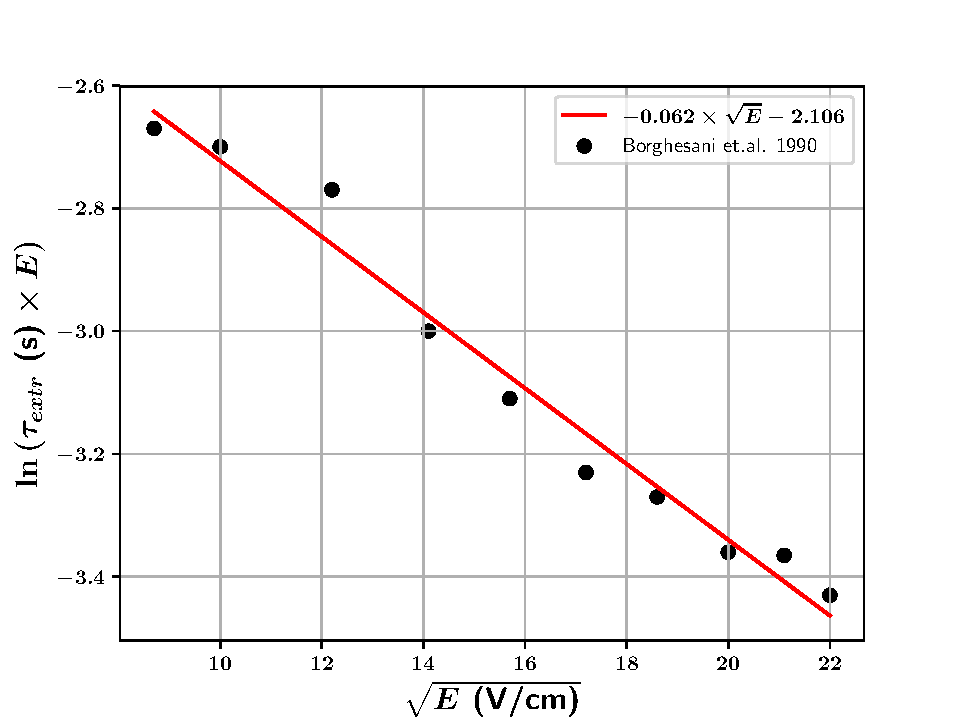
\includegraphics[width=\textwidth,keepaspectratio]{slow_time_fit.pdf}
          \caption{Les points sont les mesures faites dans \cite{Borghesani1990}, la ligne rouge est l'ajustement à ces données de la formule proposée dans le même article, donnée dans la légende.}
        \end{subfigure}
        \begin{subfigure}[t]{0.5\textwidth}
          \flushright        
          \captionsetup{width=.95\linewidth}
          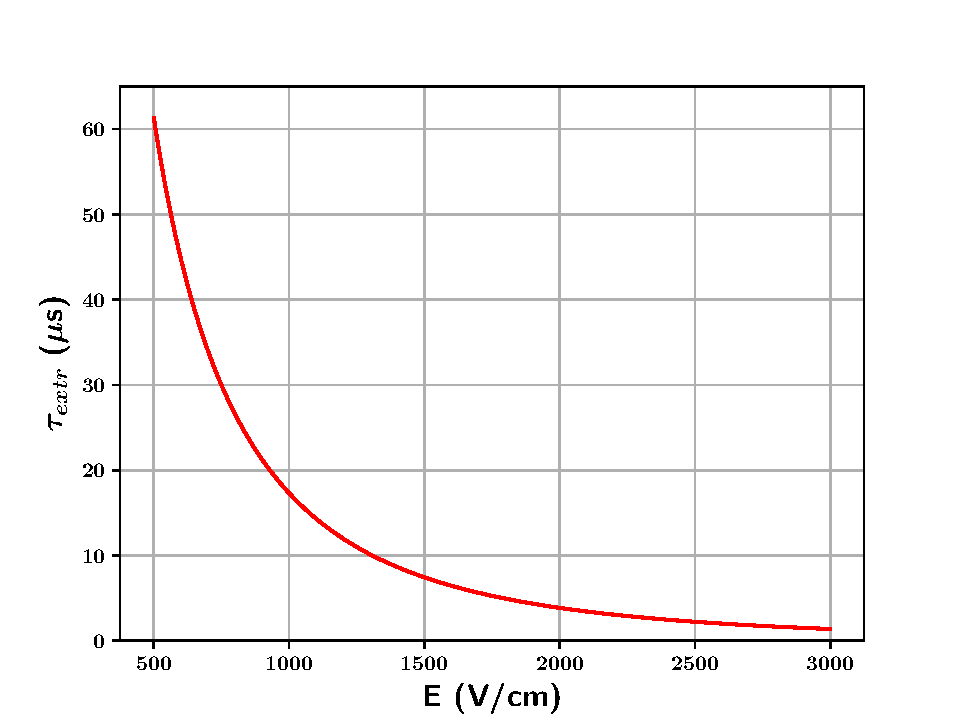
\includegraphics[width=\textwidth,keepaspectratio]{slow_time_vs_E.pdf}
          \caption{Temps caractéristique de la composante lente de l'extraction en fonction du champ électrique dans le liquide, à partir de l'ajustement fait dans la figure de gauche.}
        \end{subfigure}
        \caption[Temps caractéristique l'extraction en fonction du champ électrique]{\label{fig::slow_time_vs_E}Temps caractéristique de la composante lente de l'extraction en fonction du champ électrique dans le liquide.}
      \end{figure}

      Avant de pouvoir être amplifiés, les électrons doivent sortir du liquide et atteindre le gaz. Il est nécessaire pour cela d'appliquer un champ électrique dans le liquide, dit "champ d'extraction" d'environ \SI{2}{\kilo\volt\per\centi\meter}. En effet, une étude faite par Gushchin et al. en 1982\cite{guschin} a montré que l'extraction des électrons se fait en deux temps. Une composante "rapide", où l'électron est extrait en moins de \SI{0.1}{\micro\second}, et une composante lente.  La \autoref{fig::guschin} montre la proportion d'électrons de chaque composante en fonction du champ électrique. La proportion d'électrons dans la composante rapide croît avec le champ, et on peut y ajuster un polynôme d'ordre 4. La proportion d'électrons dans la composante lente peut être ajustée par une gaussienne, et devient négligeable au-delà de \SI{2.5}{\kilo\volt\per\centi\meter}. La somme des deux composantes n'est pas nécessairement égale à 1, indiquant que des électrons peuvent ne pas être extraits du tout. Le nombre d'électrons extraits par la composante lente en fonction du temps suit une exponentielle décroissante, dont le temps caractéristique peut être de l'ordre de la microseconde\cite{Borghesani1990}, ce qui peut entraîner un étalement en temps du signal. Ce temps caractéristique décroît avec le champ d'extraction, comme l'a mesuré Borghesani et al.\cite{Borghesani1990} (voir \autoref{fig::slow_time_vs_E}). %La \autoref{fig::extraction} montre le calcul de l'étalement en temps de l'extraction d'une charge initiale ponctuelle pour plusieurs champs d'extractions. 
      %TODO rajouter la convolution à la réponse de l'électronique et conclure sur la perte due à l'extraction

      Les mesures faites dans le prototype de \threeL{} ont, de plus, mis en évidence un plateau du gain en fonction de ce champ d'extraction à plus de \SI{2}{\kilo\volt\per\centi\meter} (voir \autoref{fig::wu_extr}). Ce phénomène, reproduit par des simulations et discuté en \autoref{sec::efficacites}, est du à la perte d'électrons sur le \gls{lem} avant amplification à cause de la forme des lignes de champs. Un champ d'extraction nominal de \SI{2}{\kilo\volt\per\centi\meter} est donc préconisé pour les \glspl{dlartpc} de \gls{wa105}. Ce champ est créé par une grille située sous l'interface liquide-gaz, une différence de potentiel entre cette grille et la face basse du ou des \glspl{lem} permet de générer le champ d'extraction. Pour une différence de potentiel $\Delta V_{LEM-grille}$, une distance $d_l$ entre la grille et l'interface et une distance $d_g$ entre l'interface et le \gls{lem}, les champs dans le liquide et le gaz sont donnés par
      \begin{eqnarray}\label{eq::fields_liquid_gas}
          E_{liquide} = \frac{\Delta V_{LEM-grille}}{d_l(1-\frac{\epsilon_l}{\epsilon_g}) + (d_l+d_g)\frac{\epsilon_l}{\epsilon_g}} \\ 
          E_{gaz} = \frac{\Delta V_{LEM-grille} - E_{liquide} \times d_l}{d_g}
        \end{eqnarray}
      où $\epsilon_l$ et $\epsilon_g$ sont les constantes diélectriques de l'argon liquide et gazeux respectivement. Dans le design des \glspl{dlartpc} de \gls{wa105} et du prototype de \threeL{}, la grille est située \SI{1}{\centi\meter} sous le \gls{lem} et l'interface au milieu entra la grille et le \gls{lem}. Pour atteindre un champ de \SI{2}{\kilo\volt\per\centi\meter}, il est alors nécessaire d'appliquer une différence de potentiel de \SI{2.5}{\kilo\volt}.

      \begin{figure}[htbp]
        \centering
        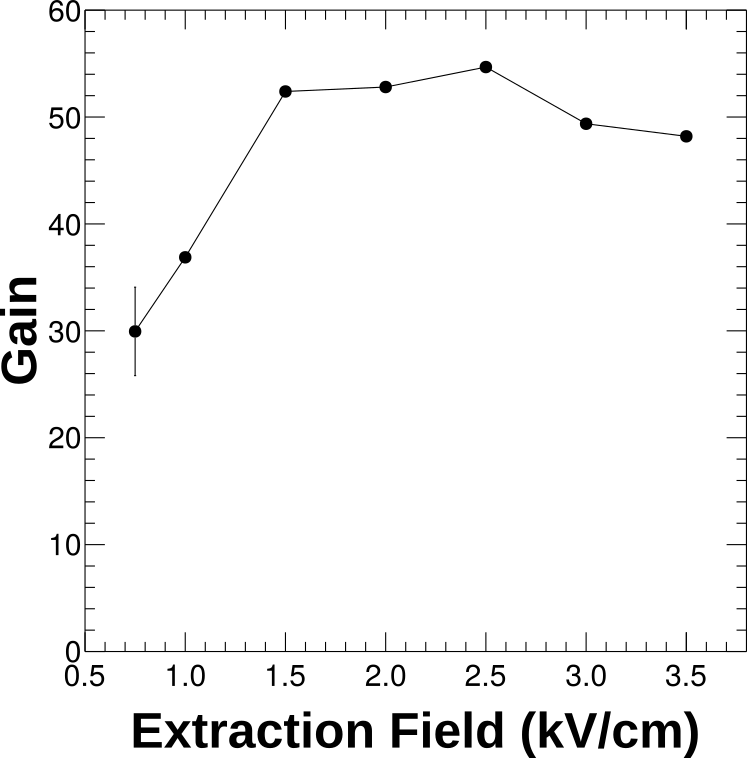
\includegraphics[width=0.6\textwidth,keepaspectratio]{wu_extr.png}
        \caption[Effet du champ d'extraction sur le gain mesuré dans le prototype de \threeL{}]{\label{fig::wu_extr}Effet du champ d'extraction sur le gain mesuré dans le prototype de \threeL{}\cite{Wu2017}.}
      \end{figure}

    \subsection{Lecture des électrons}\label{sec::induction}
    
      Dans les \glspl{dlartpc} de \gls{wa105} et du prototype de \threeL{}, après extraction et amplification, les électrons sont dirigés vers les anodes par un champ électrique dit d'induction, créé par une différence de potentiel entre le haut des \glspl{lem} et les anodes. Un champ d'induction plus grand permet de récupérer une plus grande partie des électrons sortant du \gls{lem} (voir \autoref{sec::efficacites}), cependant des contraintes techniques empêchent d'augmenter infiniment ce champ tout en restant stable. Une valeur nominale de \SI{5}{\kilo\volt\centi\meter} est utilisée. Les anodes segmentées (voir \autoref{fig::anode}) sont de même dimension que les \glspl{lem}, et ont des canaux de lecture larges d'environ \SI{3}{\milli\meter}. Les deux vues de ces anodes partagent la charge équitablement entre elle. Les anodes sont situées \SI{2}{\milli\meter} au dessus des \glspl{lem}.

    \subsection{État de l'art}\label{sec::state_of_the_art}

      \begin{table}[]
        \centering
        \begin{tabular}{|ll||ll|}
          \hline
          \multicolumn{2}{|c||}{LEM} & \multicolumn{2}{c|}{Anode} \\ \hline \hline
          Épaisseur FR4 & \SI{1}{\milli\meter} & Capacitance & \SI{140}{\pico\farad\per\meter} \\
          Diamètre des trous & \SI{0.5}{\milli\meter} & Largeur des canaux & \SI{3}{\milli\meter} \\
          Géométrie & Héxagonale &  &  \\
          RIM & \SI{40}{\micro\meter} &  &  \\ \hline
        \end{tabular}
        \caption[Caractéristiques des LEMs et anodes utilisé dans le \threeL{}]{\label{tab::lem_anode}Caractéristiques des LEMs et anodes préconisées par les résultats du prototype de \threeL{}}
      \end{table}

      \begin{figure}[htbp]
        \centering
        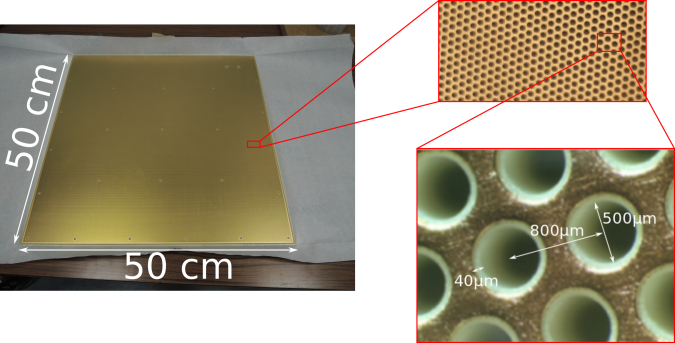
\includegraphics[width=\textwidth,keepaspectratio]{LEM_zoom.png} 
        \caption[Photo d'un amplificateur d'électron]{Photo d'un \gls{lem} avec agrandissement de la disposition en nid d'abeille des trous d'amplification. Le modèle présenté est celui utilisé dans le prototype de \TOO{}, ceux utilisés dans le prototype de \threeL{} mesuraient $10\times\SI{10}{\centi\meter\squared}$.}
        \label{fig::lem}
      \end{figure}

      \begin{figure}[htbp]
        \centering
        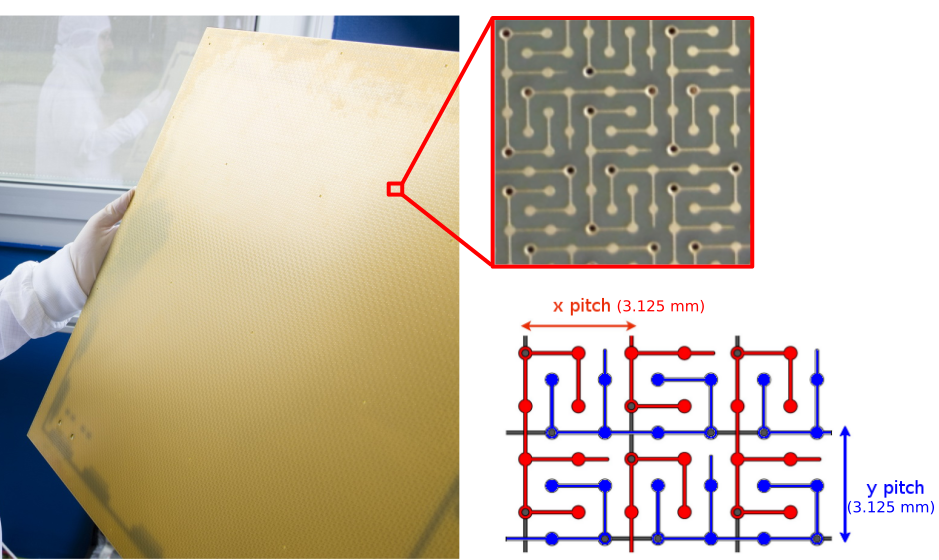
\includegraphics[width=0.8\textwidth,keepaspectratio]{anode.png}
        \caption[Photo et schéma d'une anode]{Photo et schéma d'une anode de $50\times\SI{50}{\centi\meter\squared}$. Le design vient des études du prototype de \threeL{}\cite{Wu2017,Cantini2013} et permet un partage égal de la charge entre les deux vues tout en minimisant la capacitance.}
        \label{fig::anode}
      \end{figure}

      \begin{figure}[htbp]
        \begin{subfigure}[t]{0.48\textwidth}
          \flushleft
          \centering
          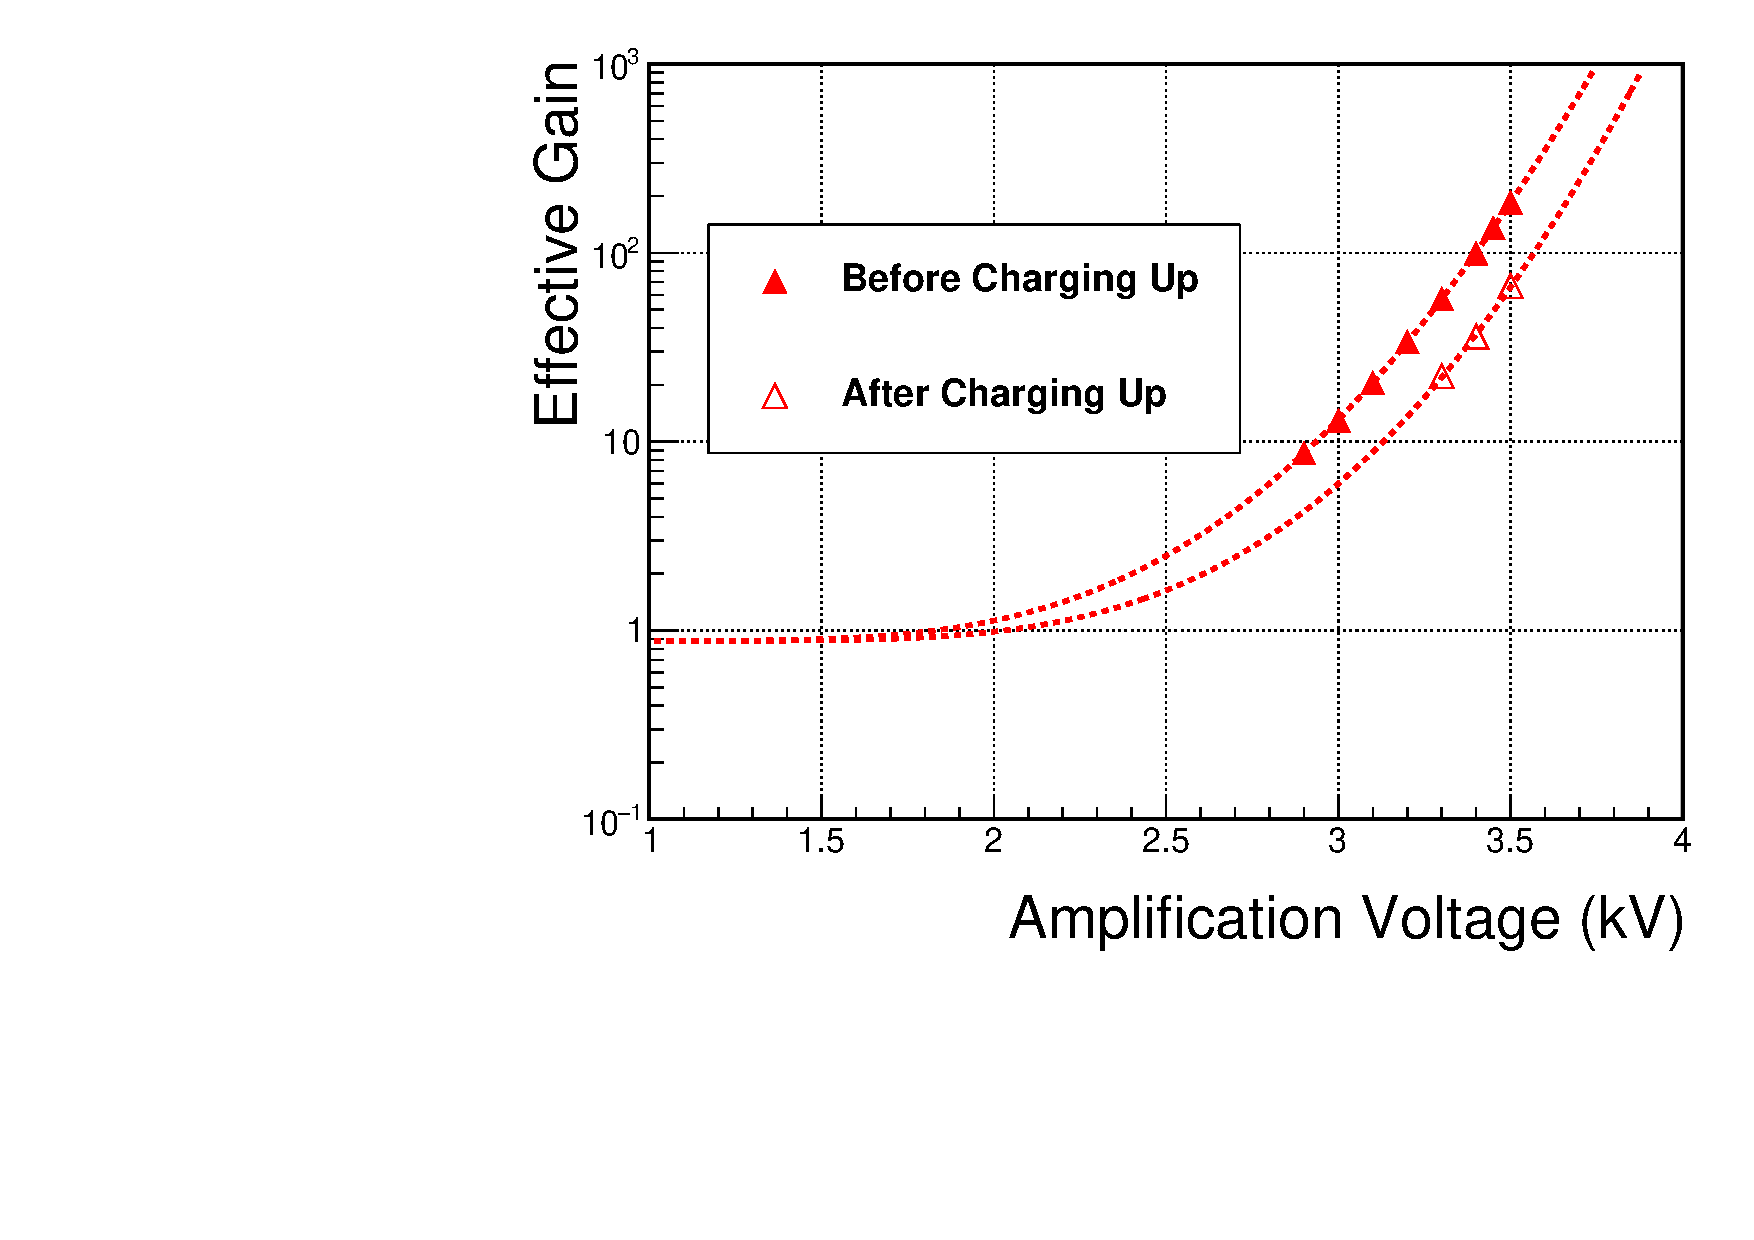
\includegraphics[width=\textwidth,keepaspectratio]{gain_3L.pdf}
        \end{subfigure}\hfill
        \begin{subfigure}[t]{0.48\textwidth}
          \flushleft
          \centering
          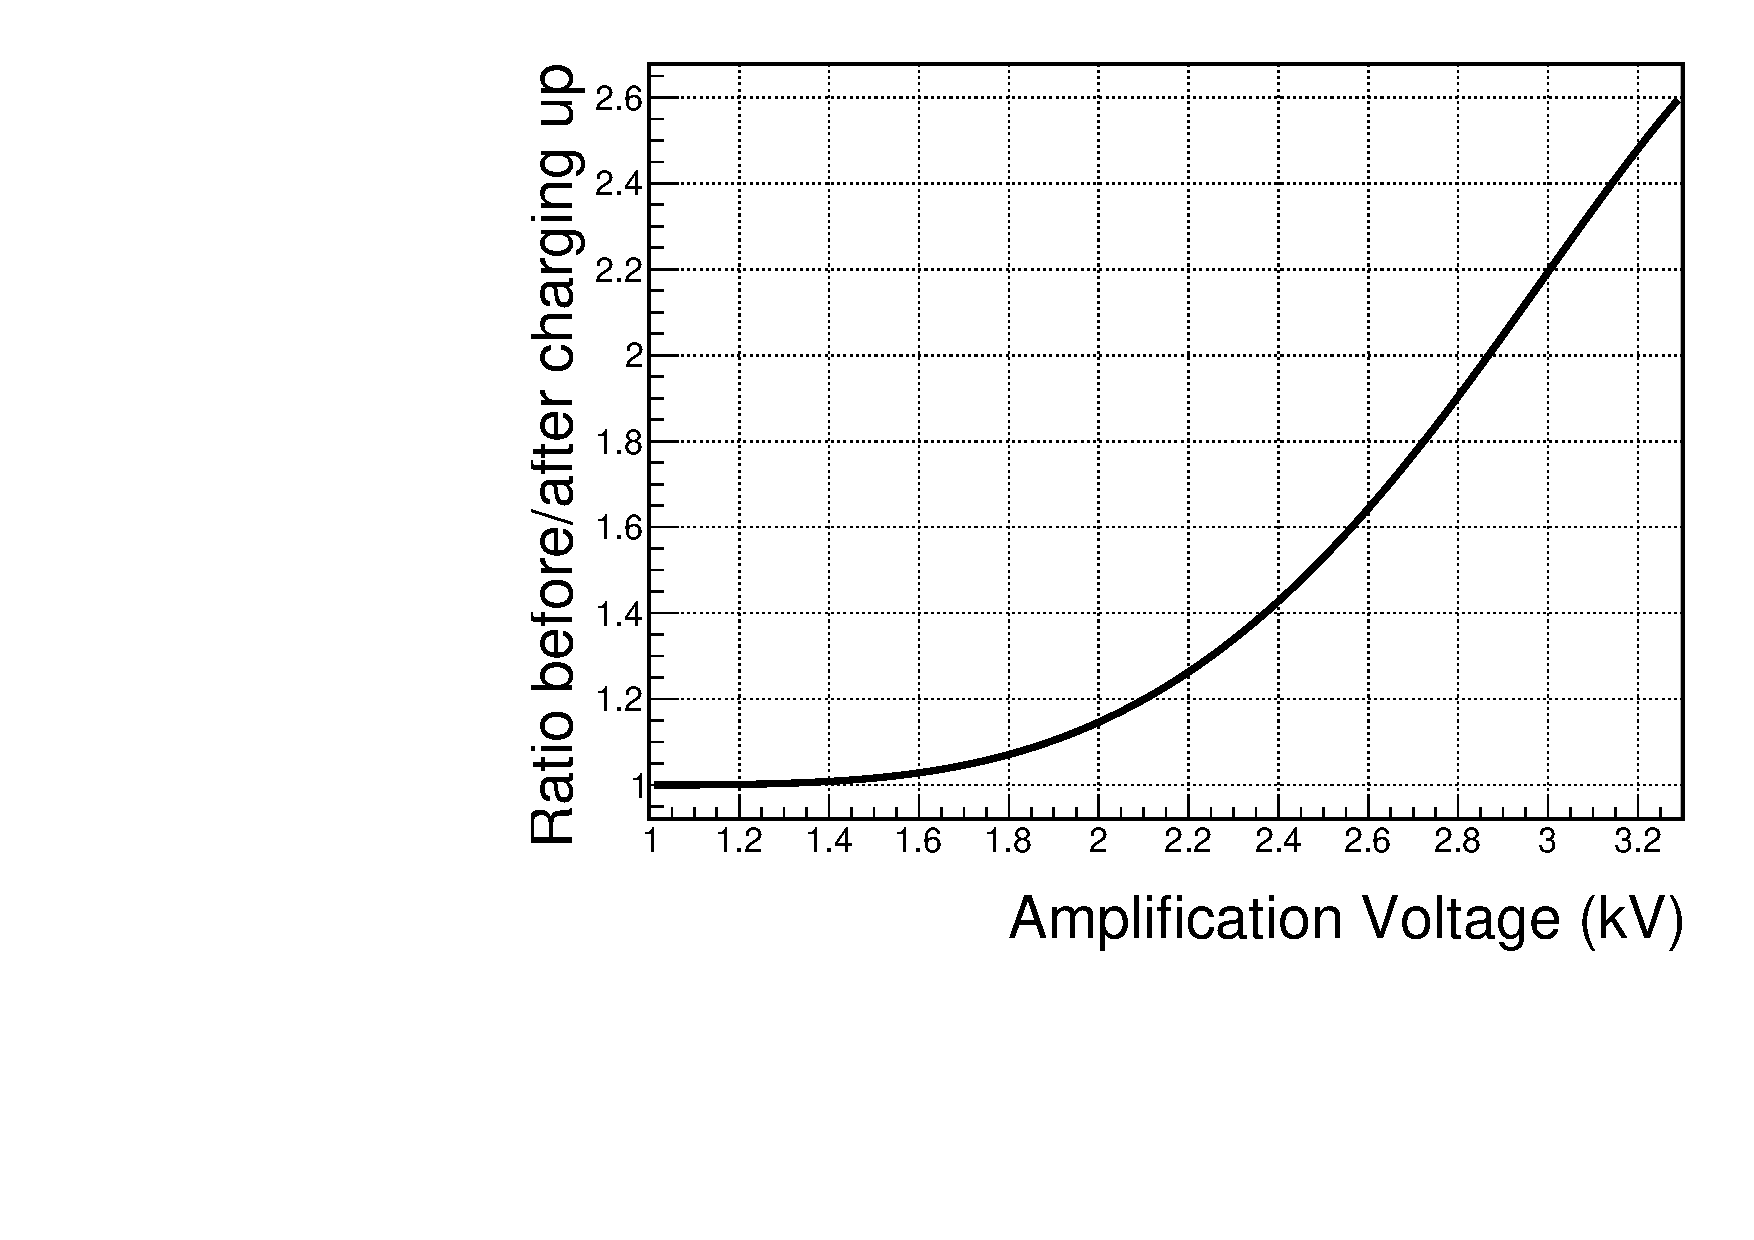
\includegraphics[width=\textwidth,keepaspectratio]{ratio.pdf}
        \end{subfigure}
        \caption[Gain en fonction du potentiel mesuré par le prototype de \threeL{}]{
        \label{fig::3L_gain}Gauche : gain en fonction de la tension d'amplification, mesuré par le prototype de \threeL{} avant et après charging up, ajusté par l'équation \eqref{eq::gain_eff}. Droite : Ratio calculé entre le gain avant et après charging up avec les résultats de cet ajustement.}
      \end{figure}

      Une étude de 2008 sur les \glspl{lem}\cite{Breskin2008} a montré qu'il est nécessaire de munir ces derniers de RIMs protecteurs : autour des trous d'amplifications, un anneau sans cuivre doit être présent afin d'assurer la stabilité en tension (voir \autoref{fig::lem}). Sans ça, des effets de pointes provoquent des décharges fréquentes et empêchent d'atteindre les tensions requises pour avoir des gain conséquents. Par la suite, le prototype de \threeL{}\cite{Cantini2013,Cantini2014} a permis d'étudier de nombreux aspects de la technologie \gls{dlartpc}. Il a mesuré le gain effectif en fonction du champ d'amplification, montrant qu'un gain de 20 est atteignable pour un champ d'amplification de \SI{31}{\kilo\volt\centi\meter} (voir \autoref{fig::3L_gain}). Il a également étudié le comportement du gain en fonction du temps. Ce dernier décroît jusqu'à atteindre une valeur plateau $G_{\infty}$ suivant la loi
      \begin{equation}
        G_{eff}(t) = \frac{G_{eff}^{\infty}}{1-\left(1-\frac{G_{eff}^{\infty}}{G_{eff}^0}\right)\times e^{-t/\tau_{cu}}}.
      \end{equation}
      où $G_{eff}^{\infty}$ est le gain effectif quand $t\to\infty$ et $G_{eff}^0$ est le gain à $t=0$. Ce phénomène, appelé charging up, est due à l'accumulation d'électrons sur le \gls{fr4} à l'intérieur des trous d'amplifications. Ceci vient du fait que les lignes de champs peuvent traverser le \gls{fr4}, à cause du RIM. Cette accumulation va peu à peu modifier le champ électrique dans le trou, jusqu'à ce que les lignes de champ ne traversent plus le \gls{fr4}. À ce moment là, le gain est stationnaire. La valeur du temps caractéristique $\tau_{cu}$ va dépendre, pour un design de \gls{lem} fixé, du taux de charges arrivant, et donc de la longueur de la zone de dérive et de l'exposition. Dans le cas du \threeL{}, qui avait une dérive de \SI{21}{\centi\meter} et était exposé aux rayons cosmiques en surface, ce temps était de l'ordre de la demi journée. Il a également été observé que, l'or de la décharge d'un \gls{lem}, la zone autour de la décharge voit son gain revenir à $G_{eff}^0$, ce qui veut dire qu'une décharge "nettoie" le \gls{lem} des électrons accumulés sur le \gls{fr4} autour de la zone de décharge (quelques centimètres carrés).  Le charging up diminue le gain en diminuant le champ d'amplification. Le gain en fonction de l'amplification étant exponentiel, il est attendu que le ratio entre le gain avant et après charging up augmente avec le champ d'amplification. Dans le papier du \threeL{} de 2014, trois mesures de gain ont été faites après charging up. Un ajustement à ces données du gain attendu \eqref{eq::gain_eff} permet, avec l'ajustement du même gain aux données avant charging up, d'estimer la variation de ce ratio avec le champ d'amplification. La \autoref{fig::3L_gain} montre le résultat de cet ajustement, qui est utilisé en \autoref{sec::result_gain} pour comparer les résultats du \TOO{} à ceux du \threeL{}.

      Le prototype de \threeL{} a utilisé ces mesures de gains pour déterminer les caractéristiques optimales des \glspl{lem}. Il a montré qu'à une tension d'amplification fixée, une épaisseur plus grande de \gls{fr4} correspond à un temps de charge $\tau_{cu}$ plus grand. Une disposition hexagonale des trous permet d'atteindre des gains plus grands qu'une disposition en carrés. Un diamètre des trous plus grand permet une meilleure stabilité en tension du \gls{lem} durant une exploitation de plusieurs jours, mais implique une baisse plus importante du gain durant le charging up du \gls{lem}. La même étude a déterminé la géométrie des anodes permettant un partage équitable de la charge entre les deux vues, facilitant la reconstruction, tout en réduisant la capacitance et donc le bruit électronique sur les canaux de lecture. Une asymétrie entre les vues de \numprint{0.7}\,\% et une capacitance de \SI{140}{\pico\farad\per\meter} (correspondant à un bruit électronique de 1240 électrons sur des canaux de \SI{1}{\meter}) ont été atteints par le modèle de l'anode présentée en \autoref{fig::anode}. Les caractéristiques des \glspl{lem} et des anodes sont résumées dans le \autoref{tab::lem_anode}.

%      Des simulations ont également été faites afin d'étudier la diffusion des électrons à travers le \gls{lem}\cite{Wu2017}, et ont servi à définir la largeur de \SI{3}{\milli\meter} des canaux de lecture des anodes. Les coefficients de diffusion dans l'argon gazeux peuvent être jusqu'à 100 fois supérieurs à ceux de l'argon liquide, et sur le demi millimètre de dérive entre l'interface liquide-gaz et le \gls{lem} une distribution ponctuelle d'électrons sera gaussienne avec un écart type transverse (perpendiculaire au sens de dérive)de \SI{0.4}{\milli\meter} et un écart type longitudinale (parallèle au sens de dérive) de \SI{0.2}{\milli\meter}. Le passage de ce même nuage d'électrons à travers le \gls{lem} augmentera peu l'écart type transverse (90\,\% des électrons se trouvent à \SI{1.6}{\milli\meter} du centre de la distribution), mais peut tripler l'écart type longitudinal. Ces mêmes études ont montré que le milieu du nuage électronique met environ \SI{0.9}{\micro\second} pour atteindre le \gls{lem} depuis l'interface liquide-gaz sous un champ d'extraction de \SI{2.5}{\kilo\volt\per\centi\meter}, et \SI{0.4}{\micro\second} pour traverser le \gls{lem} et atteindre l'anode. La vitesse de dérive dans le gaz fait que l'étalement longitudinal du signal, qui correspond à la durée entre la sortie du premier électron du \gls{lem} et l'arrivée du dernière à l'anode, est autour de \SI{0.4}{\micro\second} également.

%      A noter que ces simulations n'ont été faites qu'à un ensemble de champs électriques fixés, et que l'étalement en temps peut dépendre des champs, tout particulièrement du champ d'extraction.
    
  \section{Les processus physiques dans l'argon liquide}\label{sec::lar}

%    \begin{figure}[htbp]
%      \begin{subfigure}[t]{0.57\textwidth}
%        \flushleft
%        \centering
%        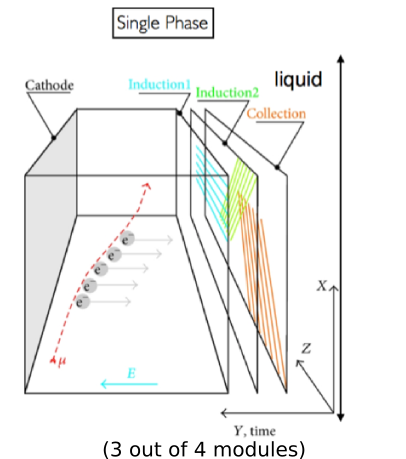
\includegraphics[width=\textwidth,keepaspectratio]{lartpc.png}
%      \end{subfigure}
%      \begin{subfigure}[t]{0.43\textwidth}
%        \flushright
%        \centering
%        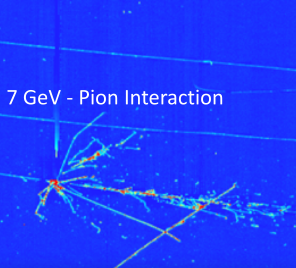
\includegraphics[width=\textwidth,keepaspectratio]{SP_evt.png}
%      \end{subfigure}
%      \caption[Schéma d'une chambre à projection temporelle à argon liquide et exemple d'événement vue par \protosp{}.]{\label{fig::lartpc}Schéma d'une chambre à projection temporelle à argon liquide (gauche) et événement mesuré dans le prototype de \protosp{} (droite) correspondant à une interaction d'un proton de \SI{7}{\giga\eV} (zoom).}
%    \end{figure}
%    Le principe de la \acrfull{tpc} a été proposé pour la première fois en 1974 par D.R.~Nygren\cite{Nygren1974}. Il s'agit d'un volume rempli de gaz ou de liquide à travers lequel est appliqué un champ électrique appelé champ de dérive. Une particule chargée traversant le milieu l'ionise, laissant des paires électron-ion dans son sillage. Le champ de dérive sépare les ions, qui vont dériver vers la cathode, des électrons, qui vont dériver vers l'anode. Si le milieu est gazeux, les électrons peuvent être amplifiés grâce à un fort champ électrique, pouvant augmenter le signal jusqu'à un facteur 1000. La lecture des électrons peut se faire en utilisant plusieurs plans de détections. Avec au moins deux plans, l'information $x$ et $y$ de la trace peut être reconstruite. L'information $z$ peut être obtenu grâce au temps de dérive et à la vitesse de dérive des électrons dans le milieu. L'énergie déposée par la particule est proportionnelle à la charge collectée, et l'information de la perte d'énergie par unité de longueur permet d'identifier les particules grâce à la formule de Bethe-Bloch (voir \autoref{sec::MPV}). Il est également possible de magnétiser la \gls{tpc} afin d'identifier le signe de la charge des particules et de mesurer leur impulsion. La \autoref{fig::lartpc} illustre le principe de fonctionnement d'une \gls{tpc} détectant une interaction neutrino dans de l'argon liquide.

%    La \gls{tpc} a plusieurs avantages:
%    \begin{itemize}
%      \item[$\bullet$] Toutes les interactions ont lieu dans un volume homogène et continue, sans zones mortes.
%      \item[$\bullet$] Le gaz ou le liquide remplissant ce volume est à la fois la cible et le milieu de détection.
%      \item[$\bullet$] L'information 3D des traces est reconstruite sans ambiguïté.
%      \item[$\bullet$] Il est possible de séparer plusieurs traces même quand la densité de trace est importante, permettant l'étude d'interactions complexes.
%      \item[$\bullet$] Il est possible de reconstruire la charge déposée dans le milieu et d'utiliser le dépôt d'énergie par unité de longueur pour identifier les particules.
%      \item[$\bullet$] Une \gls{tpc} peut être magnétisée afin d'identifier le signe des particules chargées et de mesurer leur impulsion.
%    \end{itemize}
    
%    La première \gls{tpc} a été utilisée dans le complexe de détecteur PEP-4 pour étudier des collisions électrons-positrons. La forme cylindrique est la plus adaptée pour les expériences de collisionneur, et la plus grosse \gls{tpc} à gaz actuellement en service est celle de l'expérience ALICE sur le LHC. Pour une expérience de physique des neutrinos, la forme cylindrique n'apporte aucun avantage et le gaz n'est pas un milieu suffisamment dense pour avoir une nombre d'interactions conséquent. En 1977, C.~Rubbia propose donc la \acrfull{lartpc} \cite{Rubbia1977} spécifiquement pour l'étude des neutrinos et autres événements rares.
    
%  \section{La TPC à argon liquide}\label{sec::lartpc}
    
%    La \autoref{fig::lartpc} montre le principe de fonctionnement de la \gls{lartpc} simple phase, donc sans amplification de la charge. L'ionisation de l'argon par une particule chargée va générer, en plus des paires électron-ion, une grande quantité de photons de \SI{128}{\nano\meter}. Ces photons, détectés par des \glspl{pmt}, servent de déclencheur pour l'enregistrement des événements. La dérive des électrons se fait ensuite horizontalement grâce à un champ de dérive de \driftfield{} sur deux fois \SI{1.5}{\meter} vers le ou les \glspl{crp}. Un \gls{crp} est constitué de trois plans verticaux de fils conducteurs. Les deux premiers lisent la charge de manière non destructive, par induction. La charge est ensuite collectée sur le troisième plan. Un seul volume compris entre un plan de lecture et une cathode est représenté sur la \autoref{fig::lartpc}, mais une grande \gls{lartpc} peut être un assemblage de plusieurs de ces volumes. C'est le cas de \gls{icarus} et \protosp{}, l'expérience de prototypage de la technologie \gls{lartpc} simple phase au CERN. Dans ce prototype, qui a commencé à prendre des données en faisceau en 2018, deux volume ayant chacun une longueur de dérive de de \SI{3.6}{\meter} sont présents.
%
%    La version "double phase", prototypée par le projet \protodp{}, prendra des données cosmiques à partir de l'été 2019, et pourra peut être prendre des données de faisceau après le second arrêt long du CERN qui a commencé fin 2018 et finira fin 2020. Dans cette version, schématisée par la \autoref{fig::dlartpc}, une fine couche d'argon gazeux est maintenue à la surface de l'argon liquide. La dérive se fait donc verticalement, sur \SI{6}{\meter}, avec la cathode placée en bas du volume d'argon liquide et les \glspl{crp} placés dans la phase gazeuse. Ces \glspl{crp} ne sont plus des plans de fils verticaux : ils sont horizontaux et sont constitués d'une grille d'extraction, d'amplificateurs d'électrons et d'anodes segmentées. La grille, une maillage 2D de fils conducteurs, sert à extraire les électrons de la phase liquide à la phase gazeuse. Les amplificateurs, des \glspl{pcb} de \SI{1}{\milli\meter} d'épaisseur, sont capables de fournir un gain effectif stable autour de 20 d'après les premiers prototypes de cette technologie\cite{Cantini2014}. Les anodes segmentées, des \glspl{pcb} pourvues de deux ensembles de canaux perpendiculaires, sont capables de reconstruire l'information $x/y$ des événements. Comme dans la version simple phase, l'information en $z$ est donnée par le temps de dérive et la vitesse de dérive des électrons dans l'argon liquide.

    \subsection{Pourquoi l'argon liquide?}
      L'argon liquide a de nombreux atouts à être utilisé dans une \gls{tpc}\cite{Rubbia1977} :
      \begin{itemize}
        \item[$\bullet$] Il ne capture pas les électrons de dérive, permettant des distances de dérive de plusieurs mètres et une grande précision sur la mesure de la charge déposée.
        \item[$\bullet$] La mobilité des électrons est suffisamment grande et leur diffusion suffisamment faible atteindre une précision millimétrique sur des dérives de l'ordre du mètre.
        \item[$\bullet$] Il est inerte. Il n'y a donc pas de phénomène de vieillissement des éléments présents dans le volume à cause de l'argon.
        \item[$\bullet$] Il est dense, augmentant la probabilité de détection d'événements rares comparé aux \gls{tpc} à gaz.
        \item[$\bullet$] Il scintille lors de l'ionisation, et est transparent à sa propre scintillation, ce qui permet à cette scintillation d'être utilisée temps initiale pour les événements, voir comme déclencheur.
        \item[$\bullet$] Il est peu cher et abondant.
      \end{itemize}
      Les propriétés physico-chimique de l'argon sont résumées dans le \autoref{tab::Ar}.
      \begin{table}[htpb]
        \centering
        \begin{tabular}{|l|c|}
          \hline
          \textbf{Propriété} & \textbf{Symbol, valeur et/ou unité} \\ \hline \hline
          Numéro atomique & $Z$, 18 \\
            \specialrule{.01em}{.0em}{.0em}
          Masse atomique & $A$, \SI{39.948}{\gram\per\mole} \\
            \specialrule{.01em}{.0em}{.0em}
          \begin{tabular}[c]{@{}l@{}}Température d'ébulition\\ à pression atmosphérique\end{tabular} & \SI{87.303}{\kelvin} \\
            \specialrule{.01em}{.0em}{.0em}
          \begin{tabular}[c]{@{}l@{}}Température de fusion\\ à pression atmosphérique\end{tabular} & \SI{83.8}{\kelvin} \\
            \specialrule{.01em}{.0em}{.0em}
          Densité (liquide) & $\rho$, \SI{1.3973}{\gram\per\centi\meter\cubed} \\
            \specialrule{.01em}{.0em}{.0em}
          Point triple & \SI{83.8059}{\kelvin}, \SI{0.68891}{\bar} \\
            \specialrule{.01em}{.0em}{.0em}
          \begin{tabular}[c]{@{}l@{}}constante diélectrique\\ du gaz (du liquide)\end{tabular} & $\epsilon_{g}(\epsilon_{l})$, \numprint{1.000516}(\numprint{1.504}) \\
            \specialrule{.01em}{.0em}{.0em}
          \begin{tabular}[c]{@{}l@{}}Énergie d'ionisation\\ du gaz (du liquide)\end{tabular} & $W$, \SI{26.4}{\eV} (\SI{23.6}{\eV}) \\
            \specialrule{.01em}{.0em}{.0em}
          \begin{tabular}[c]{@{}l@{}}Énergie d'excitation\\ moyenne du liquide\end{tabular} & $I$, \SI{188}{\eV} \\
            \specialrule{.01em}{.0em}{.0em}
          \begin{tabular}[c]{@{}l@{}}Longueur d'onde de \\ scintillation\end{tabular} & \SI{128}{\nano\meter} \\
%            \specialrule{.01em}{.0em}{.0em}
%        \begin{tabular}[c]{@{}l@{}}Longueur de diffusion\\ de Rayleigh (liquide, \SI{128}{\nano\meter})\end{tabular} & \SI{90}{\centi\meter} \\ 
          \hline
        \end{tabular}
        \caption[Propriété physiques et chimiques de l'argon]{\label{tab::Ar}Propriété physiques et chimiques de l'argon.}
      \end{table}

    \subsection{De l'ionisation de l'argon à la dérive des électrons}\label{sec::ionisation}
        %https://lar.bnl.gov/properties/

        Le nombre d'électrons issus de l'ionisation va dépendre de l'énergie déposée dans le milieu, qui va dépendre de l'impulsion de la particule incidente. Un détecteur segmenté comme les \glspl{dlartpc} de \gls{wa105} va s'intéresser à la charge reçue dans chaque canal de lecture, et donc au dépôt d'énergie par unité de longueur, décrit dans la prochaine sous-section. Après ionisation, une fraction des électrons produits vont se recombiner avec des ions. Il faut prendre en compte ce phénomène dans la reconstruction de l'énergie déposée. Le facteur de recombinaison, définie comme la fraction d'électrons restant après recombinaison, dépend du champ appliqué et de l'énergie déposée (voir équation \eqref{eq::birk}). Cette recombinaison produit également des photons de \SI{128}{\nano\meter}\footnote{La scintillation est également due à l'excitation d'atomes d'argon par la particule incidente sans création de paires électron-ion.}, qui résulte de la désexcitation d'atomes d'argon ayant réabsorbé un électron d'ionisation et qui peuvent être utilisés comme temps initial ou déclencheur. Lors de leur dérive, les électrons peuvent être absorbés par des impuretés présentes dans l'argon liquide, principalement O$_2$, H$_2$O et CO$_2$. Le nombre d'électrons survivants suit une loi exponentielle décroissante, caractérisée par un temps de vie effectif des électrons. \gls{icarus} a mesuré un temps de vie de \SI{15}{\milli\second}\cite{Antonello2014} en observant l'atténuation du signal avec la distance de dérive. Le prototype de \protosp{} a quant à lui déduit un temps de vie de \SI{7}{\milli\second}. Le \autoref{tab::lifetime} présente la fraction d'électrons restante pour ces deux durées de vie et pour différentes longueurs de dérive. Durant leur dérive, les électrons vont subir de nombreuses diffusions, résultant en un étalement du signal le long de la dérive et dans le plan perpendiculaire à la dérive. La densité d'électrons suit alors une distribution normale décrites par l'équation \eqref{eq::diffusion}. L'importance de la diffusion va dépendre du champ électrique et de la température. La suite de cette section décrit en détail les processus résumés dans ce paragraphe, et le \autoref{tab::muon} donne les valeurs importantes liées à ces mêmes processus pour des muons au minimum d'ionisation, qui peuvent être utilisés pour calibrer et/ou étudier le gain d'une \gls{dlartpc}. 

      \subsubsection{Énergie déposée dans l'argon liquide}

        \begin{table}[htpb]
          \centering
          \begin{tabular}{|cl|l|cl|}
            \cline{1-2} \cline{4-5}
            Symbol & Définition &  & Symbol & Définition \\ \cline{1-2} \cline{4-5} 
            $K$ & \begin{tabular}[c]{@{}l@{}}$4\pi N_Ar_e^2m_ec^2$,\\ \SI{0.307075}{\mega\eV\centi\meter\squared\per\mole}\end{tabular} &  & $m_ec^2$ & \begin{tabular}[c]{@{}l@{}}Masse de l'électron multiplité par \\ la célérité de la lumière,\\ \SI{0.510998928(11)}{\mega\eV}\end{tabular} \\
            $r_e$ & \begin{tabular}[c]{@{}l@{}}Rayon classique de l'électron,\\ \SI{2.8179403267(27)}{\femto\meter}\end{tabular} &  & $I$ & Énergie d'exitation moyenne, \si{\eV} \\
            $N_A$ & \begin{tabular}[c]{@{}l@{}}Nombre d'Avogadro,\\ \SI{6.02214129(27)e23}{\per\mole}\end{tabular} &  & $T_{max}$ & \begin{tabular}[c]{@{}l@{}}Énergie maximum transférée à \\ un électron, $\frac{2m_ec^2\beta^2\gamma^2}{1+2\gamma m_e/M +(m_e/M)^2}\si{\mega\eV}$\end{tabular} \\
            $q$ & \begin{tabular}[c]{@{}l@{}}Nombre de charge élémentaire\\ de la particule incidente\end{tabular} &  & $M$ & Masse de la particule incidente \\
            $Z$ & Numéro atomique du milieu &  & $\delta(\beta\gamma)$ & \begin{tabular}[c]{@{}l@{}}Correction due aux effets de \\ densité (voir \cite{pdg2018})\end{tabular} \\
            $A$ & Masse atomique du milieu &  & $T_{cut}$ & \begin{tabular}[c]{@{}l@{}}Coupure sur l'énergie maximum\\ transférée à un électron, \si{mega\eV}\end{tabular} \\
            $\beta$ & \begin{tabular}[c]{@{}l@{}}$v/c$ avec $v$ la vitesse de la \\ particule incidente\end{tabular} &  & $\rho$ & Densité du milieu, \si{\gram\per\centi\meter\cubed} \\
            $\gamma$ & Facteur de Lorentz, $\frac{1}{\sqrt{1-\beta^2}}$ &  & $ds$ & \begin{tabular}[c]{@{}l@{}}Distance sur laquelle la particule\\ incidente dépose de l'énergie, \si{\centi\meter}\end{tabular} \\ \cline{1-2} \cline{4-5} 
          \end{tabular}
          \caption[Paramètres utilisés dans les équations \eqref{eq::bethe_bloch}, \eqref{eq::bethe_tcut} et \eqref{eq::mpv}]{\label{tab::bethe_params}Paramètres utilisés dans les équations \eqref{eq::bethe_bloch}, \eqref{eq::bethe_tcut} et \eqref{eq::mpv}. Tableau tiré de \cite{pdg2018}.}
        \end{table}

        \begin{figure}[htbp]
          \centering
          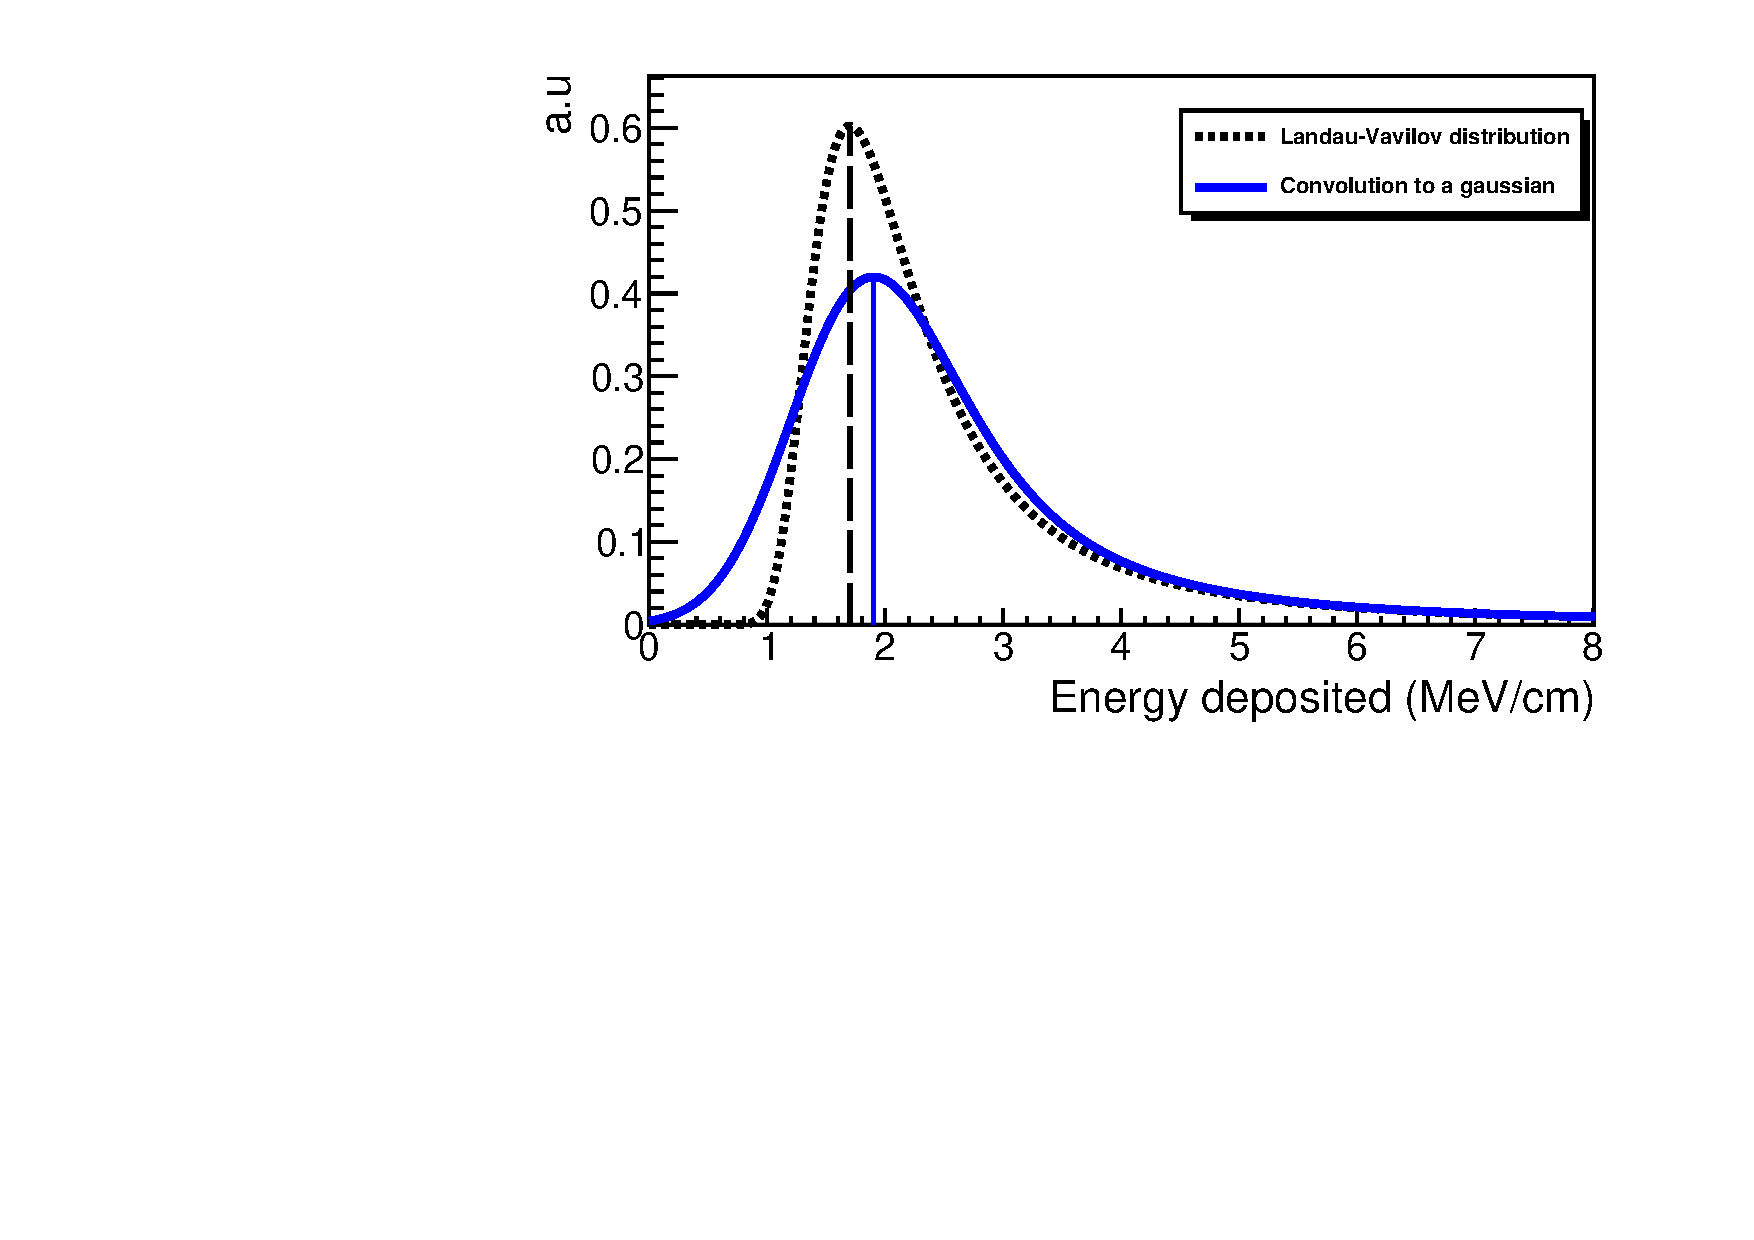
\includegraphics[width=0.8\textwidth,keepaspectratio]{langau.pdf}
          \caption[Distribution de Landau-Vavilov convoluée à une gaussienne]{\label{fig::langau}Distribution de Landau-Vavilov (pointillés noirs) convoluée à une gaussienne (trait plein bleu). Les traits verticaux indiquent les valeurs les plus probables des deux distributions.}
        \end{figure}

        Une \gls{tpc} est capable de visualiser une trace en 3D et de mesurer l'énergie déposée dans le milieu. Très souvent, il est nécessaire de pouvoir comparer la mesure de l'énergie à une prédiction (calibration, estimation de gain...). Chaque canal de lecture va mesurer la charge résultant du dépôt d'énergie d'une particule le long d'une petite distance $ds$ dans le liquide. Si l'énergie déposée sur cette distance est faible en comparaison de l'énergie totale de la particule incidente, alors cette dernière peut être considérée comme ayant une impulsion constante durant la traversée du milieu. Dans ce cas, la distribution de l'énergie déposée par unité de longueur $\frac{\Delta E}{ds}$ suivra approximativement une loi de Landau-Vavilov convoluée à une Gaussienne\cite{Bichsel2006} (c'est le cas pour un muon cosmique traversant de l'argon liquide). La \autoref{fig::langau} montre une telle distribution, avec en pointillés noirs la loi de Landau-Vavilov seule et en trait plein bleu la convolution à une gaussienne. Les traits verticaux indiquent les \glspl{mpv} des deux distributions. Cette distribution est asymétrique et tend vers l'infinie quand l'énergie déposée tend vers l'infini. De ce fait, elle n'a pas de moyenne définie. Physiquement, l'énergie déposée est finie et cette distribution est tronquée. Un spectre expérimental aura donc une moyenne mesurable. Cette moyenne ainsi que la \gls{mpv} de la Landau-Vavilov dépendent le l'impulsion de la particule incidente, et peuvent être utilisées pour calibrer le détecteur.

        L'énergie moyenne perdue par unité de longueur par une particule dans un milieu, $\frac{dE}{dx}\rvert_{moyenne}$, est appelée pouvoir d'arrêt. Dans les milieux de numéro atomique intermédiaire comme l'argon, et pour des particules ayant un $\beta\gamma$ compris entre \numprint{0.1} et \numprint{1000} (c'est le cas des muons cosmiques), ce pouvoir d'arrêt est bien décrit par la loi de Bethe-Bloch\cite{pdg2018} :
        \begin{equation}\label{eq::bethe_bloch}
          \frac{dE}{dx}\biggr\rvert_{moyenne} = -Kq^2 \frac{Z}{A\beta^2}\left[\frac{1}{2}\ln\left(\frac{2m_ec^2\beta^2\gamma^2T_{max}}{I^2}\right)-\beta^2-\frac{\delta(\beta\gamma)}{2} \right].
        \end{equation}
        Les définitions des différents paramètres de cette équation sont donnés dans le \autoref{tab::bethe_params}, les valeurs pour l'argon sont données dans le \autoref{tab::Ar}. Ce pouvoir d'arrêt dépend de l'impulsion de la particule incidente, de sa charge électrique, ainsi que du milieu traversé. Il dépend également de la masse de la particule à travers $T_{max}$, mais cette dépendance n'est visible qu'à très haute énergie\cite{pdg2018}. En pratique, à charge fixée, cette moyenne dans un milieu donné ne dépend que de l'impulsion de la particule incidente. L'allure de cette moyenne en fonction de l'impulsion pour un muon est représentée en trait pleins bleu sur la \autoref{fig::bethe_landau}. On y voit une valeur minimum à \SI{2.12}{\mega\electronvolt\per\centi\meter}, ce qui correspond à une \gls{mip}. Les autres courbes sont expliquées plus loin.

        \begin{figure}[htbp]
          \centering
          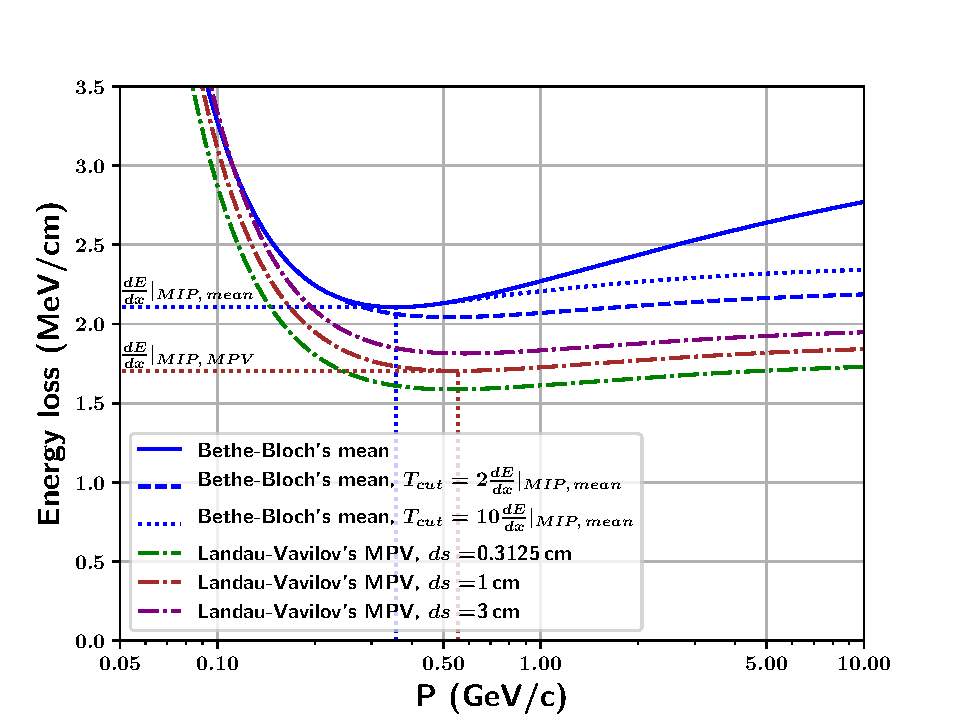
\includegraphics[width=0.8\textwidth,keepaspectratio]{dE_dx.pdf}
          \caption[Énergie perdue par unité de longueur d'une MIP en fonction de l'impulsion]{\label{fig::bethe_landau}Énergie perdue par unité de longueur par un muon dans de l'argon liquide en fonction de l'impulsion. En trait plein bleu est représentée la formule de Bethe et Bloch, résultat de l'équation \eqref{eq::bethe_bloch}, représentant l'énergie moyenne perdue par unité de longueur. Le minimum est désigné par $\frac{dE}{dx}\rvert_{MIP,\,mean}$. Les deux traits pointillés bleus représentent la formule de Bethe et Bloch avec une coupure sur l'énergie maximum transférée, résultat de l'équation \eqref{eq::bethe_tcut}. En points-tiraits de couleur sont représentés des \glspl{mpv} de la Landau-Vavilov pour plusieurs distances de dépôt d'énergie.}
        \end{figure}

        \begin{figure}[htbp]
          \centering
          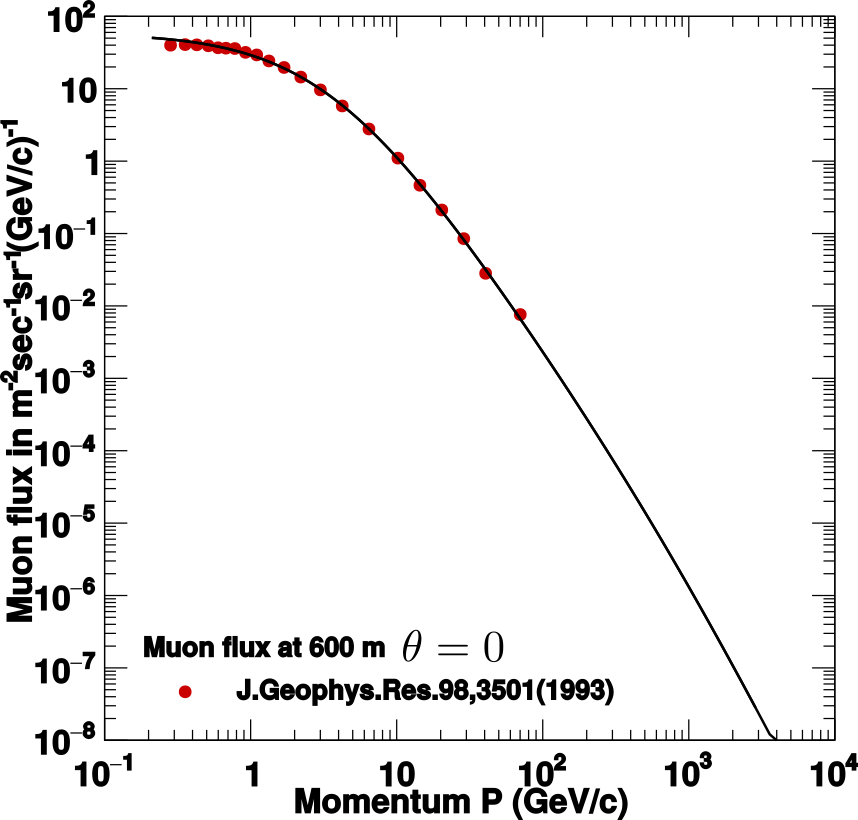
\includegraphics[width=0.7\textwidth,keepaspectratio]{muon_600m_0deg.png}
          \caption[Flux de muons cosmique sur terre]{\label{fig::muon_flux}Flux de muons cosmique sur terre, à une altitude de \SI{600}{\meter} et un angle zénithal de 0\cite{Shukla2016}. Pour comparaison, le \gls{cern} se situe entre \SI{400}{\meter} et \SI{500}{\meter}.}
        \end{figure}
        
        Dans un détecteur, si une particule incidente transfère une grande partie de son énergie à un électron, ce dernier peut ioniser le milieu à son tour et être détectable. Un tel électron est appelé $\delta-e$ (ce n'est pas un électron de dérive). S'il est discernable de la trace principale, son énergie, et donc l'énergie perdue par la particule incidente au moment de la création de ce $\delta-e$, ne figurera pas dans la distribution des $\frac{\Delta E}{ds}$\footnote{Il est cependant possible, avec un bon algorithme, d'identifier les $\delta-e$ et leur trace d'origine, et de calculer ainsi l'énergie perdue au moment de leur création.}. Dans ce cas, la moyenne de la distribution, $\frac{\Delta E}{ds}\rvert_{mean}$, sera différente du pouvoir d'arrêt $\frac{dE}{dx}\rvert_{mean}$. Il est cependant possible de modifier l'équation \eqref{eq::bethe_bloch} en y incluant une coupure sur l'énergie maximum transférée, $T_{cut}$\cite{pdg2018}. Cette coupure doit correspondre à la limite en dessous de laquelle un $\delta-e$ n'est plus discernable de la trace principale dans le détecteur et dépend donc du détecteur et de la performance des algorithmes de reconstruction. L'équation modifiée est alors :
        \begin{equation}\label{eq::bethe_tcut}
          \frac{dE}{dx}\biggr\rvert_{T\leq T_{cut}} = Kq^2 \frac{Z}{A\beta^2}\left[\frac{1}{2}\ln\left(\frac{2m_ec^2\beta^2\gamma^2T_{cut}}{I^2}\right)-\frac{\beta^2}{2}\left(1+\frac{T_{cut}}{T_{max}}\right)-\frac{\delta(\beta\gamma)}{2} \right]
        \end{equation}
        et son allure est représentée par les traits pointillés bleu sur la \autoref{fig::bethe_landau}. On voit que l'impulsion correspondant à une \gls{mip} augmente  et que le minimum diminue quand $T_{cut}$ diminue. De plus, $\frac{dE}{dx}\rvert_{T\leq T_{cut}}$ atteint un plateau, contrairement à $\frac{dE}{dx}\rvert_{mean}$.
        
        Pour s'affranchir de cette difficulté inhérente à l'estimation de $T_{cut}$, il est possible d'utiliser la \gls{mpv} de la loi de de Landau-Vavilov présente dans la distribution des $\frac{\Delta E}{ds}$. Cependant, cette valeur notée $\frac{\Delta E}{ds}\rvert_{MPV}$ ne correspond pas au maximum de la distribution des $\frac{\Delta E}{ds}$, de par la convolution à une Gaussienne. Elle doit être extraite par un ajustement. La \gls{mpv} d'une Landau-Vavilov suit l'équation\cite{pdg2018}
        \begin{eqnarray}
          \frac{dE}{dx}\biggr\rvert_{MPV} = & \xi\left[\ln(ds) + \ln\left(\frac{2m_ec^2\beta^2\gamma^2}{I}\right)+\ln(\xi/I)+j-\beta^2 - \delta(\beta\gamma)\right] \label{eq::mpv} \\
          \xi = & \frac{KZ\rho z^2}{2A\beta^2}\nonumber\\
          j = & 0.200.\nonumber
        \end{eqnarray}
        Où $z$ est la charge électrique de la particule incidente. Cette \gls{mpv} ne dépend pas de la coupure $T_{cut}$, a un minimum $\frac{dE}{dx}\biggr\rvert_{MIP,MPV}$ pour une certaine impulsion et présente un plateau à haute énergie. De plus, elle varie en $a\ln(ds)+b$. Elle est présentée en fonction de l'impulsion en \autoref{fig::bethe_landau} en points-tiraits pour plusieurs valeurs de $ds$. En vert pour $ds=\SI{0.3125}{\centi\meter}$, qui est la plus petite valeur possible dans \protodp{} et qui correspond à la taille d'une piste de lecture. En rouge pour $ds=\SI{1}{\centi\meter}$, qui est la valeur la plus souvent mesurée dans le prototype de \TOO{}, et en brun pour $ds=\SI{3}{\centi\meter}$, valeur au delà de laquelle très peu de traces sont observées dans le prototype de \TOO{}. Plus de détails sur les $ds$ mesurés dans le \TOO{} sont apportés en \autoref{sec::results-311}. On constate que l'impulsion correspondant au minimum ne dépend pas de $ds$ et vaut \SI{0.56}{\giga\eV\per c}. De plus, la variation de l'énergie déposée autour de ce minimum est faible. La majorité des muons cosmiques arrivant sur terre étant entre \SI{0.3}{\giga\eV\per c} et \SI{3}{\giga\eV\per c} (voir \autoref{fig::muon_flux}), considérer ces derniers comme étant au minimum d'ionisation est une bonne approximation et permet ainsi d'estimer le gain d'une \gls{dlartpc}. $\frac{dE}{dx}\rvert_{MPV}$ est également montrée en fonction de $ds$ en \autoref{fig::mpv_ds}. On voit qu'elle augmente d'environ 10\;\% entre \SI{0.3125}{\centi\meter} et \SI{3}{\centi\meter}.

        \begin{figure}[htbp]
          \centering
          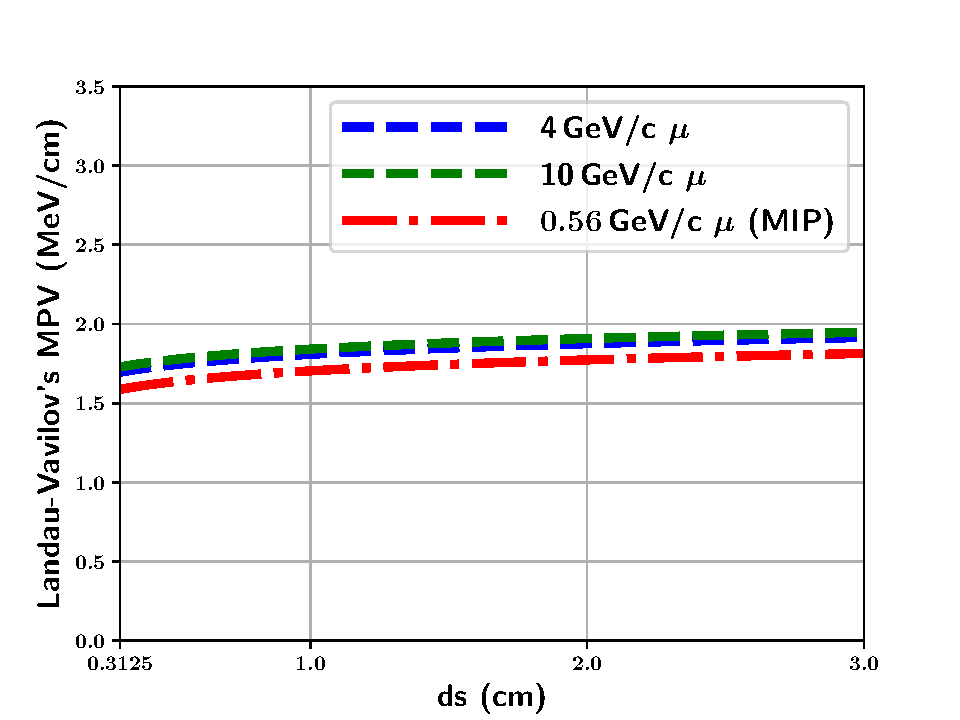
\includegraphics[width=0.8\textwidth,keepaspectratio]{MPV_vs_ds.pdf}
          \caption[Valeur la plus probable de la distribution de Landau-Vavilov en fonction de la distance de dépôt d'énergie]{\label{fig::mpv_ds}Valeur la plus probable de la distribution de Landau-Vaviloc en fonction de la distance de dépôt d'énergie, pour des muons au minimum d'ionisation et pour des muons de \SI{4}{\giga\electronvolt}.}
        \end{figure}

        Dans la suite de cette thèse, $\frac{dE}{dx}\rvert_{MPV}$ sera préférée à $\frac{dE}{dx}\rvert_{moyenne}$ et sera notée simplement appelé \gls{mpv}.

      \subsubsection{Recombinaison}\label{sec::recombinaison}

        Lors du passage d'une particule ionisante dans la matière, cette dernière va exciter et/ou ioniser les atomes du milieu en leur transférant une partie de son énergie, principalement par collision. Si l'énergie ainsi transférée lors d'une collision est supérieure à l'énergie nécessaire pour arracher un électron à l'atome, appelée énergie d'ionisation et notée $W$, un ou plusieurs électrons vont être arrachés et libérés dans le milieu. Autrement, l'atome peut se retrouver dans un état excité et devra se désexciter par rayonnement de photons.

        \begin{figure}[htbp]
          \centering
          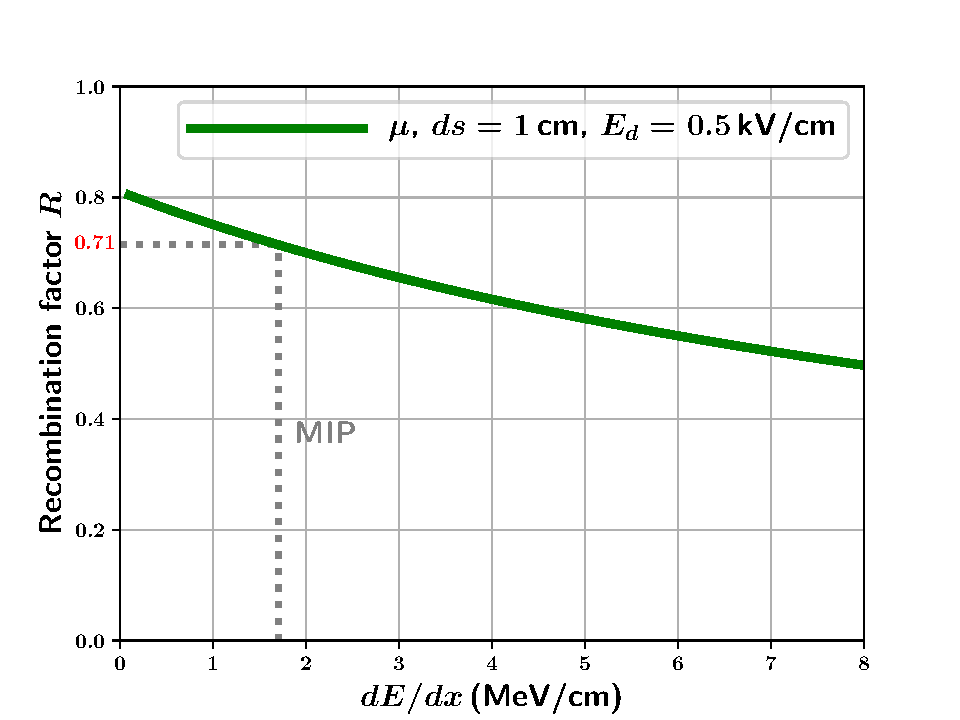
\includegraphics[width=0.8\textwidth,keepaspectratio]{R_vs_MPV.pdf}
          \caption[Facteur de recombinaison de la loi de Birk en fonction du dépôt d'énergie par unité de longueur]{\label{fig::birk}Facteur de recombinaison de la loi de Birk (équation \eqref{eq::birk}) en fonction du dépôt d'énergie par unité de longueur. La valeur indiquée par les pointillés correspond au minimum de la \gls{mpv} de la Landau-Vavilov en fonction de l'impulsion  pour un distance de dépôt d'énergie de \SI{1}{\centi\meter} (\autoref{fig::bethe_landau}).}
        \end{figure}

        Après ionisation, les électrons peuvent soit entamer leur dérive, soit être captés par un atome ionisé et se recombiner. Le nombre total d'électrons dérivant sera donc inférieur au nombre d'électrons initialement arrachés. Cette recombinaison peut être décrite par trois approches différentes, décrites dans \cite{Amoruso2004}:
        \begin{itemize}
          \item[$\bullet$] La théorie de Onsager considère la probabilité qu'a un électron de revenir à son ion d'origine. Il s'agit alors d'une loi en exponentielle décroissante dépendant de l'énergie de l'électron, avec un facteur prenant en compte l'effet du champ de dérive.
          \item[$\bullet$] La théorie de la colonne suppose une distribution en colonne des charges autour de la trace de la particule incidente. Les électrons et ions s'éloignent de la colonne sous l'effet du champ de dérive et de la diffusion. Les électrons et les ions peuvent alors se recombiner suivant les distributions des charges positives et négatives autour de la trace.
          \item[$\bullet$] Le modèle en boîte, qui reprend la théorie de la colonne mais en supposant les ions fixent et aucune diffusion.
        \end{itemize}
        La loi de Birk, énoncée par J.B. Birks en 1964\cite{Birk1964} est une approximation du modèle en colonne. Cette loi a été ajustée aux données de muons cosmiques dans l'argon liquide par \gls{icarus} en 2004\cite{Amoruso2004}. Cette loi introduit le facteur de recombinaison $R$, qui correspond au ratio entre le nombre d'électrons de dérive et le nombre d'électrons initialement arrachés au milieu. Ce facteur augmente avec le champ de dérive, puisque ce dernier favorise la séparation des ions et des électrons, mais diminue avec la quantité d'énergie déposée. Il s'écrit
        \begin{equation}\label{eq::birk}
          R=\frac{A}{1+\frac{k}{E_d \rho}\frac{dE}{dx}}
        \end{equation}
        avec $E_d$ le champ de dérive, et $A=\numprint{0.81}(5)$ et $k=\SI{0.055\pm0.005}{\kilo\volt\gram\per\centi\meter\cubed\per\mega\eV}$ d'après les ajustements fait par \gls{icarus} dans \cite{Amoruso2004}. La \autoref{fig::birk} montre la variation de $R$ en fonction de l'énergie déposée par unité de longueur dans un champ électrique de \driftfield{}. Les lignes pointillées correspondent à la \gls{mpv} d'une particule au minimum d'ionisation, qui donne $R=\numprint{0.71}$.

      \subsubsection{Photons de scintillation}

        \begin{figure}[htbp]
          \centering
          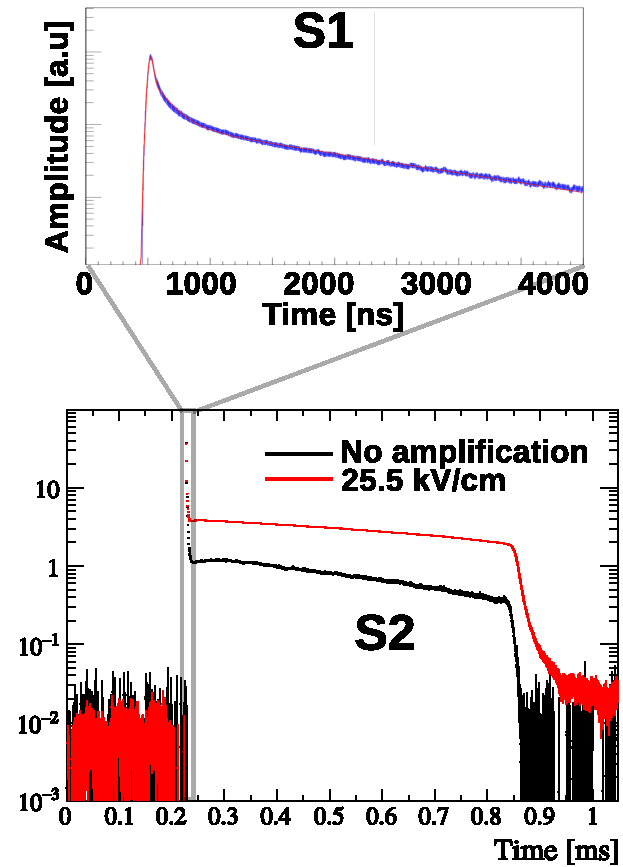
\includegraphics[width=0.8\textwidth,keepaspectratio]{scintillation.pdf}
          \caption[Scintillation dans une chambre à projection temporelle à argon liquide double phase]{\label{fig::scintillation}Scintillation vue dans le prototype de \TOO{}\cite{Aimard2018}. En noir est tracée la moyenne des mesures de 3 \glspl{pmt} en l'absence de champ d'amplification. En rouge est tracée la même mesure en présence d'un champ d'amplification. Le pic à \SI{200}{\micro\second} correspond à l'ionisation initiale, dans le liquide. Le continuum correspond à la traversée progressive des électrons dans le gaz, où une scintillation sera présente pour des champs électrique de l'ordre de \SI{2}{\kilo\volt\per\centi\meter} ou plus. La durée d'émission d'environ \SI{600}{\micro\second} correspond à la durée de dérive attendue pour des électrons parcourant \SI{1}{\meter} dans un champ de \driftfield{}.}
        \end{figure}
        
        Au moment de l'ionisation de l'argon liquide, un grand nombre de photons à \SI{128}{\nano\meter}\cite{Gedanken1972} (\SI{9.7}{\eV}) est également émis. Cette émission peut se faire de deux manières différentes :
        \begin{itemize}
          \item[$\bullet$] Un atome d'argon excité $Ar^*$ va se coupler à un atome d'argon $Ar$ pour former un dimère excité $Ar_2 ^*$. Ce dimère se scinde ensuite en deux atomes d'argon en émettant un photon $\gamma$.
          \item[$\bullet$] Un ion argon $Ar^+$ va se coupler à un atome d'argon $Ar$ pour former un dimère ionisé $Ar_2 ^+$. Ce dimère se scinde en deux après recombinaison avec un électron $e^-$. Il en résulte un atome d'argon $Ar$ et un atome d'argon très excité $Ar^{**}$. Ce dernier perd une partie de son énergie sous forme de chaleur et devient un $Ar^*$, qui va alors subir le processus précédent.
        \end{itemize} 
        Ces deux processus, résumés dans l'équation \eqref{eq::scintillations}, peuvent donner lieu à deux états différents\footnote{Chacun des deux processus peut donner les deux états.} de $Ar^*$ notés $^1\Sigma_u^+$ et  $^3\Sigma_u^+$. Le premier a un temps de désexcitation rapide, de $\sim\SI{7}{\nano\second}$, le second a un temps de désexcitation plus lent, de $\sim\SI{1600}{\nano\second}$\cite{Hitachi1983}.
        \begin{equation} \label{eq::scintillations}
            \begin{split}
            \text{Excitation}\begin{cases}
            Ar^* + Ar & \to Ar_2^* \\
            Ar_2^* & \to 2Ar + \gamma\\
            \end{cases} \\
            \text{Recombinaison}\begin{cases}
            Ar^+ + Ar & \to Ar_2^+  \\
            Ar_2^+ + e^- & \to Ar^{**}+Ar  \\
            Ar^{**} & \to Ar^*+\text{chaleur}  \\
            Ar^* + Ar & \to Ar_2^*  \\
            Ar_2^* & \to 2Ar + \gamma \\
            \end{cases}
            \end{split}
        \end{equation}

        Le temps de dérive des électrons dans l'argon liquide étant de l'ordre de la milliseconde, une émission de photons quelques nanosecondes après l'ionisation peut servir à définir le temps initial de l'événement, où $t_0$. Celui-ci servira à mesurer le temps d'arrivée de chaque électron, permettant de mesurer la distance au \gls{crp} de la trace. A ces fins, il est nécessaire de pouvoir détecter les photons émis lors de l'ionisation. Si le but est simplement de détecter l'émission des photons sans chercher à reconstruire leur origine avec précision (ce qui suffit quand on utilise les photons comme déclencheurs), les différentes diffusions de ces photons dans l'argon n'ont pas d'importance. En revanche, l'absorption des photons par l'argon ou les impuretés peut avoir un impact négatif. Baldini et al. on étudié l'absorption d'UV dans l'argon solide en 1962 \cite{Baldini1962}, et on trouvé qu'en dessous de \SI{11}{\eV}, les photons ne sont pas absorbés. L'énergies de photons de \SI{128}{\nano\meter} étant de \SI{9.7}{\eV}, l'argon est transparent à sa propre scintillation. Les impuretés en revanche peuvent être nuisibles. L'étude de R. Acciarri et al. de 2009\cite{Acciarri2009} montre que la présence de dioxygène ou de diazote peut entraîner une diminution de la quantité de photons détectés. Cette diminution reste cependant inférieure au pourcent en dessous d'une concentration de \SI{100(1000)}{ppb} de dioxygène(diazote). Les puretés mesurées par \gls{icarus}\cite{Antonello2014} et \protosp{} sont inférieures qu \si{ppb}, l'absorption de photons par les impuretés n'impact donc pas l'efficacité de déclenchement.

        Dans le cas d'une \gls{dlartpc}, une seconde scintillation a lieu lors de l'amplification du signal dans l'argon gazeux. La distribution temporelle de l'émission de $\gamma$ dans le prototype de \TOO{} est présentée en \autoref{fig::scintillation}. Le pic à \SI{200}{\micro\second} correspond à la scintillation dans le liquide, le continuum correspond à la scintillation dans le gaz, qui a lieu dès \SI{2}{\kilo\volt\per\centi\meter}. Un gain (en rouge sur la figure) entraîne comme attendu une émission plus importante de photons.

      \subsubsection{Vitesse de dérive des électrons}\label{sec::vitesse_derive}

        \begin{figure}[htbp]
          \centering
          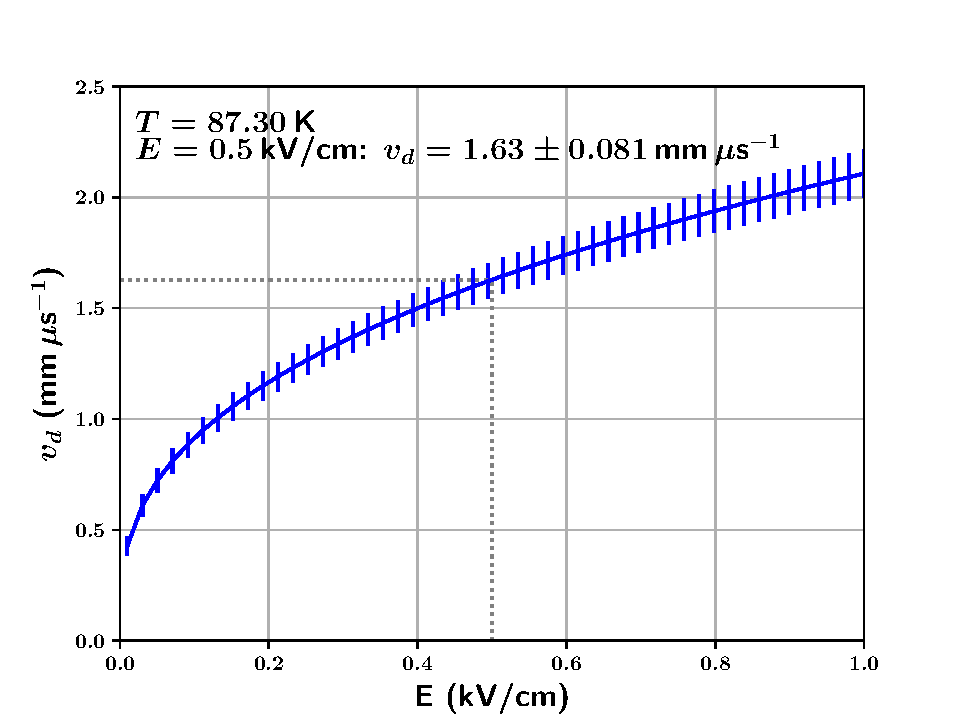
\includegraphics[width=0.8\textwidth,keepaspectratio]{vd.pdf}
          \caption[Vitesse de dérive des électrons dans de l'argon liquide en fonction du champ électrique]{\label{fig::velocity}Vitesse de dérive des électrons dans de l'argon liquide en fonction du champ électrique. La courbe est obtenue à partir de l'équation \eqref{eq::velocity} et des ajustements fait par Walkowiak et al.\cite{Walkowiak2000}.}
        \end{figure}

        La vitesse de dérive $v_d$ d'un électron dans l'argon liquide dépend du champ de dérive $E_d$ et de la température $T$ du milieu. Elle peut être paramétrisée par l'équation empirique suivante\cite{Gonidec1996}
        \begin{equation}\label{eq::velocity}
          v_d = \left(1+P_1(T-T_0)\right)\times\left(P_3E\ln\left(1+\frac{P_4}{E}\right)+P_5E^{P_6}\right) + P_2(T-T_0)
        \end{equation}
        Walkowiak et al.\cite{Walkowiak2000} ont mesuré cette vitesse et y ont ajusté avec la formule précédente en choisissant comme température de référence $T_0=\SI{90.371}{\kelvin}$.%, obtenant les coefficients présentés en \autoref{tab::fit_par}. 
        La \autoref{fig::velocity} montre la vitesse en fonction du champ électrique à \SI{87.3}{\kelvin}. A \driftfield{}, elle vaut $\SI{1.63\pm0.081}{\milli\meter\per\micro\second}$.
%        \begin{table}[htpb]
%          \centering
%          \begin{tabular}{ccc}
%          $P_1$ & = & $\SI{-0.01481\pm0.00095}{\per\kelvin}$ \\
%          $P_2$ & = & $\SI{-0.0075\pm0.0028}{\per\kelvin}$ \\
%          $P_3$ & = & $\SI{0.141\pm0.023}{\centi\meter\per\kilo\volt}$ \\
%          $P_4$ & = & $\SI{12.4\pm2.7}{\kilo\volt\per\centi\meter}$ \\
%          $P_5$ & = & $\SI{1.627\pm0.078}{(\kilo\volt\per\centi\meter)^{-P_6}}$ \\
%          $P_6$ & = & $\numprint{0.317}\pm\numprint{0.021}$ \\
%          \end{tabular}
%          \caption{\label{tab::fit_par}Paramètres de l'équation \eqref{eq::velocity}, venant de l'ajustement fait dans \cite{Walkowiak2000}.}
%        \end{table}

      \subsubsection{Pertes dues aux impuretés lors de la dérive}\label{sec::purity}
        
        Les impuretés électronégatives (O$_2$, H$_2$O, CO$_2$, N$_2$O) présentes dans l'argon peuvent capturer une partie des électrons de dérive. A chaque type d'impureté de concentration $N_i$ peut être associé un taux d'attachement $k_{s,i}$, et le nombre d'électrons en fonction du temps $N(t)$ suit alors l'équation différentielle\cite{Buckley1989}
        \begin{eqnarray}\label{eq::e_lifetime}
          N(t) = & -\sum_{i} k_{s,i}N_i N(t)\\
          \Rightarrow N(t) = & N_0\textbf{e}^{-t_d/\tau_e}=N_0\textbf{e}^{-d/(v_d\tau_e)}\label{eq::losses} \\
          \text{avec } \tau_e = & 1/(\sum_{i} k_{s,i}N_i)
        \end{eqnarray}
        où $\tau_e$ est le temps de vie de l'électron dans le milieu, qui peut être mesuré en regardant l'atténuation du signal en fonction du temps de dérive, $d$ est la distance parcourue dans le milieu et $v_d$ est la vitesse de dérive des électrons dans le milieu.

        En supposant que les seules impuretés présentes sont les molécules de dioxygène, on peut écrire $\tau = \frac{1}{k_{s,O_2} N_{O_2}}$. L'étude de Bakale et al. de 1976\cite{Bakale1976} donne $k_{s,O_2}=\SI{7.43}{\liter\per\mole\per\second}$ dans un champ de dérive de \driftfield{}. On peut alors relier la concentration de molécules de dioxygène en ppb, $\rho_{O_2}=N_{O_2}/N_{Ar}$, avec le temps de vie de l'électron ($N_{Ar}$ est le nombre de moles d'argon liquide dans un litre et est égale à $\rho/A$) : 
        \begin{equation}\label{eq::purity}
          \tau(\si{\micro\second}) = \frac{10^6}{N_{Ar}\times \rho_{O_2}(\si{ppb}) \times k_{s,i} \times 10^{-9}} = \frac{\numprint{385}}{\rho_{O_2}(\si{ppb})}.
        \end{equation}
        \gls{icarus} a mesuré un temps de vie de \SI{15}{\milli\second}\cite{Antonello2014}, correspondant à \SI{0.0257}{ppb}. Le prototype simple phase de \protosp{}, muni d'instruments permettant de mesurer la pureté de l'argon, a mesuré une concentration d'impuretés de \SI{0.055}{ppb}, correspondant à un temps de vie de \SI{7}{\milli\second}. Le \autoref{tab::lifetime} présente les fractions d'électrons restants pour ces différents temps de vie pour plusieurs longueurs de dérive, en supposant un champ de dérive de \driftfield{}.

        A partir d'ici, il est possible d'estimer la charge attendue au \gls{crp} par unité de longueur. Le tableau \autoref{tab::muon} montre que, en supposant que les muons sont au minimum d'ionisation et en utilisant la \gls{mpv} de la distribution de Landau-Vavilov, la charge attendue est de \SI{7.63}{\femto\coulomb\per\centi\meter}.

        \begin{table}[]
          \centering
          \begin{tabular}{|l|rrrr|}
            \hline
            \multicolumn{1}{|c|}{\multirow{2}{*}{\textbf{Durée de vie}}} & \multicolumn{4}{c|}{\textbf{$N/N_0$ après dérive}} \\
             & \SI{1}{\meter} & \SI{3}{\meter} & \SI{6}{\meter} & \SI{12}{\meter} \\ 
            \hline
            \hline
            \SI{7}{\milli\second} (\SI{0.055}{ppb}) & \numprint{0.92} & \numprint{0.77} & \numprint{0.59} &  \numprint{0.35} \\
            \specialrule{.01em}{.0em}{.0em}
            \SI{15}{\milli\second} (\SI{0.0257}{ppb}) & \numprint{0.96} & \numprint{0.88} & \numprint{0.78} &  \numprint{0.61} \\ \hline
          \end{tabular}
          \caption[Pertes dues aux impuretés]{\label{tab::lifetime} Électrons restants après dérive pour les durées de vie mesurées par le prototype de \protosp{} (\SI{7}{\milli\second}) et par \gls{icarus} (\SI{15}{\milli\second}), dans un champ de dérive de \driftfield{}.}
        \end{table}


        \begin{table}[]
          \centering
          \begin{tabular}{|l|r|}
            \hline
            $\frac{dE}{dx}\rvert_{MPV}(\frac{dE}{dx}\rvert_{mean})$(\si{\mega\eV\per\centi\meter}) & \numprint{1.70}(\numprint{2.12}) \\
            $R$ & \numprint{0.71}(\numprint{0.70}) \\
            \begin{tabular}[c]{@{}l@{}}Électrons arrivant\\ au \gls{crp}\end{tabular} & \numprint{51100}(\numprint{62900}) \\
            Charge (\si{\femto\coulomb\per\centi\meter}) & \numprint{8.26}(\numprint{11.0})  \\
            Signal/Bruit (sans gain) & $>13(16)$  \\
            \hline
          \end{tabular}
          \caption[Charge par unité de longueur attendue au \gls{crp} pour un muon au minimum d'ionisation dans l'argon liquide]{\label{tab::muon} Calcul de la charge par unité de longueur attendue, avant dérive (i.e avant absorption par d'éventuelles impuretés), pour un muon au minimum d'ionisation dans l'argon liquide, avec un champ de dérive de \driftfield{}. Une distance de dépôt d'énergie de \SI{1}{\centi\meter} est utilisée pour calculer la \gls{mpv}. Aucune coupure sur l'énergie maximum transférée n'est appliquée pour le calcul de l'énergie moyenne. La valeur de \SI{23.6}{\eV} de l'énergie d'ionisation dans l'argon liquide est utilisée pour calculer le nombre d'électrons. Le rapport signal sur bruit est calculé en supposant une répartition égale des charges entre les vues des anodes et un bruit électronique inférieur à \numprint{2000} électrons, correspondant à la capacitance des anodes du prototype de \TOO{}.}
        \end{table}
        
%        \cite{Buckley1989} : $\tau = \frac{1}{k_s N_s}$ avec $k_s\sim \SI{e11}{\liter\per\mole\per\second}$ et $N_s=$ concentration $O_2$ équivalente $=\rho_{O_2}\times N_{Ar}$, avec $\rho_{O_2}=[O_2]$ en particule d'$O_2$ par particule d'argon et $N_{Ar}$ le nombre de mole d'argon liquide par litre.\\
%        $N_{Ar}=\rho/A$ avec $A$ la masse atomique de l'argon liquide. $N_{Ar}=\rho/A = 1395.4/39.948 = \SI{34.9304}{\mole\per\liter}$.\\
%        $\Rightarrow \tau(\si{\micro\second}) = \frac{10^6}{3493.04\rho_{O_2}[\si{ppb}]} = \frac{286.2835}{\rho_{O_2}[\si{ppb}]}$. En prenant une meilleure lecture du graph de \cite{Bakale1976} on trouve plutôt $k_s=\SI{7.43e10}{\liter\per\mole\per\second}$. On a alors $\tau(\si{\micro\second}) = \frac{10^6}{3493.04\rho_{O_2}[\si{ppb}]} = \frac{385.31}{\rho_{O_2}[\si{ppb}]}$

      \subsubsection{Diffusion durant la dérive}\label{sec::diffusion}

        Durant leur dérive dans l'argon liquide, les électrons vont être déviés à cause des nombreuses collisions qu'ils vont effectuer avec les atomes du milieu. Cette diffusion est un phénomène aléatoire qui suit deux distributions gaussiennes : une correspondant à la diffusion dans le plan transverse à la direction de dérive, à laquelle on associe le coefficient de diffusion $D_T$, et une correspondant à la diffusion longitudinale dans le sens de la dérive, à laquelle on associe le coefficient de diffusion $D_L$. En prenant en compte les pertes dues aux impuretés et en notant $n(x,y,z,t_d)$ la densité d'électron en un point à un instant donné, on peut écrire l'équation : 
        \begin{eqnarray}
          n(x,y,z,t_d) = & \frac{n_0}{\sqrt{4\pi D_T t_d}\sqrt{4\pi D_L t_d}}\exp\left(-\frac{(z-d)^2}{4D_L t_d}\right)\exp\left(-\frac{x^2+y^2}{4D_T t_d}\right)\exp\left(-\frac{d}{v_d\tau}\right) \label{eq::diffusion} \\
%          \sigma_L(d) = & \sqrt{4\pi D_Ld/v} \label{eq::sigmaL}\\
%          \sigma_L(d) = & \frac{2\left(d^2 v^2 - 3D_L(-3D_L  + \sqrt{D_L^2 + d^2v^2}) -dv(-4D_L + \sqrt{D_L^2+d^2v^2})\right)}{v^4} \label{eq::sigmaL}\\
%          \sigma_T(d) = & \sqrt{4\pi D_Td/v} \label{eq::sigmaT}
          \sigma_L(d) \simeq & \sqrt{2 D_L d/v} \label{eq::sigmaL} \\
          \sigma_T(d) = & \sqrt{2 D_T d/v} \label{eq::sigmaT}
        \end{eqnarray}
        où $n_0$ est la densité initiale, $t_d$ le temps de dérive, $x$ et $y$ les coordonnées dans le plan perpendiculaire, $z$ la coordonnée dans le sens de la dérive, $v_d$ la vitesse de dérive et $d$ la coordonnées $z$ du milieu du nuage d'électrons. Dans une \gls{lartpc}, les pertes dues aux impuretés sont suffisamment faibles pour considérer la distribution gaussienne en temps. A un champ de dérive fixé, on peut alors exprimer les écarts types de cette distribution en fonction de la distance de dérive, suivant les équations \eqref{eq::sigmaL} et \eqref{eq::sigmaT}. Une étude de Li et al. de 2016\cite{Li2015} a mesuré, pour un champ de dérive de \driftfield{}, $D_L=\SI{7.2}{\centi\meter\squared\per\second}$, et a extrapolé à partir de données existantes la valeur de $D_T=\SI{12.0}{\centi\meter\squared\per\second}$, correspondant à des écarts types de \SI{0.94}{\milli\meter} et \SI{1.2}{\milli\meter} respectivement pour une distance de dérive de \SI{1}{\meter}. %La \autoref{fig::diffusion} montre l'allure du nuage d'électron après une dérive de \SI{1}{\meter}, \SI{3}{\meter} et \SI{6}{\meter}. Les ellipses en pointillés sont à trois écarts types. L'échelle de couleur n'est pas respectée afin de rendre visible le nuage à \SI{6}{\meter}.

    


\FloatBarrier

\printbibliography